\chapter{Data PreProcessing}

\section{Data Types and Properties}
Attribute values are assigned to an attribute for a particular object. It is useful to remember the difference between attributes and attribute values, as the same attribute can be mapped to different attribute values (for instance, height can be measured in feet or meters). Moreover, different attributes can be mapped to the same set of values (for example, both ID and age can be integers).

There are 2 main attribute types:
\begin{itemize}
    \item \textbf{Categorical (Nominal):} for instance ID numbers, eye color.
    \item \textbf{Ordinal:} for instance time, count, grades. A set of ordered attribute values.
\end{itemize}

The main difference between these 2 attribute types resides in the properties of the corresponding attribute values:
\begin{itemize}
    \item \textbf{Nominal (Categorical) Attribute Property:} Distinctness, operator ($=$).
    \item \textbf{Ordinal Attribute Properties:} Distinctness and Order, operators ($<$, $=$, $>$).
\end{itemize}

Moreover, there are Discrete and Continuous Attributes:
\begin{itemize}
    \item \textbf{Discrete Attribute:} finite set of values, often represented as integer variables. Binary attributes are a special case of discrete attributes.
    \item \textbf{Continuous Attribute:} real numbers as attribute values. In practice, real values can only be measured and represented using a finite number of digits.
\end{itemize}

Regarding Data Types we have:
\begin{itemize}
    \item \textbf{Tabular Data:} collection of records, each of them characterized by a fixed set of attributes.
    \item \textbf{Document Data:} semi-structured or unstructured textual data.
    \item \textbf{Graph Data:} for instance the World Wide Web.
    \item \textbf{Ordered Data:} for instance spatio-temporal data or genomic sequences.
\end{itemize}

\begin{table}[h]
    \centering
    \begin{tabular}{@{}lll@{}}
        \toprule
        \textbf{Tipo di attributo} & \textbf{Proprietà / operatori} & \textbf{Esempi} \\
        \midrule
        Nominale (categorico) & Distinzione ($=$) & ID, colore degli occhi \\
        Ordinale & Distinzione e ordine ($<$, $=$, $>$) & Voti, taglie S/M/L \\
        \midrule
        Discreto & Insieme finito, spesso interi & Conteggi, binari (0/1) \\
        Continuo & Numeri reali (cifre finite) & Altezza, temperatura \\
        \midrule
        \multicolumn{3}{@{}l}{\textbf{Tipi di dati}} \\
        Tabellari & Record con attributi fissi & Dataset clienti \\
        Documenti & Testo semi/non strutturato & Articoli, email \\
        Grafi & Nodi e collegamenti & World Wide Web \\
        Ordinati & Sequenze spazio-temporali & Genoma, serie storiche \\
        \bottomrule
    \end{tabular}
    \caption{Riepilogo di attributi e tipi di dati}
\end{table}

\subsection{Data Quality}
Each dataset comes with data quality issues, represented by:
\begin{itemize}
    \item \textbf{Noise and Outliers:} Noise refers to the modification of original values, for instance noise can be introduced in the data recording process. It is important to note that noise is considered to be randomly distributed. On the other hand, outliers are data objects with characteristics that are considerably different from most of the other data in the dataset. Outliers can be noise that interferes with the data analysis, or they can also be the goal of the data analysis.
    \item \textbf{Missing Values:} either the information is not collected or some attributes may not be applicable to all cases. Missing values must be handled by eliminating them, estimating them or ignoring them during the analysis.
    \item \textbf{Duplicate Data:} the dataset may include data objects that are duplicates, or almost duplicates, of one another. It is a major issue when merging data from heterogeneous sources, and Data Cleaning is needed.
\end{itemize}

\section{Similarity and Dissimilarity in Data}
\textbf{Similarity} is the numerical measure of how alike two data objects are. It is a metric that often falls in the $[0,1]$ range and is higher when objects are more alike. \textbf{Dissimilarity} is the numerical measure of how different 2 data objects are. It is lower when objects are more alike and is often a \textbf{distance metric}.

\subsection{Similarity and Dissimilarity for Simple Attributes}
A \textbf{dissimilarity} $d(x,y)$ is a numerical measure of how \emph{different} two data objects are: it is $0$ when the objects are identical and grows as they become more different. A \textbf{similarity} $s(x,y)$ measures how \emph{alike} two objects are: it is usually bounded in $[0,1]$, with $1$ meaning identical. The two notions are complementary, so similarity is typically obtained by transforming dissimilarity.
 
For simple attributes (1 dimension), the appropriate measure depends on the attribute type, since each type supports different operations:
 
\begin{center}
    \small
    \renewcommand{\arraystretch}{1.4}
    \begin{tabular}{|l|p{4.6cm}|p{5.2cm}|}
    \hline
    \textbf{Attribute Type} & \textbf{Dissimilarity} & \textbf{Similarity} \\
    \hline
    Nominal & $d=0$ if $x=y$; \newline $d=1$ if $x\neq y$ & $s=1$ if $x=y$; \newline $s=0$ if $x\neq y$ \\
    \hline
    Ordinal & $d=\dfrac{|x-y|}{n-1}$ \newline (values mapped to integers $0$ to $n-1$, where $n$ is the number of values) & $s=1-d$ \\
    \hline
    Interval or Ratio & $d=|x-y|$ & $s=-d$, \quad $s=\dfrac{1}{1+d}$, \quad $s=e^{-d}$, \newline $s=1-\dfrac{d-\min d}{\max d-\min d}$ \\
    \hline
    \end{tabular}
\end{center}
 
\paragraph{Nominal attributes.} Only the equality operator is meaningful, so two values are either identical or different: there is no notion of ``more different''. For example, $d(\text{red},\text{red})=0$, while $d(\text{red},\text{blue})=d(\text{red},\text{green})=1$.
 
\paragraph{Ordinal attributes.} Values have an order, so some pairs are farther apart than others. The values are first mapped to consecutive integers $0,\dots,n-1$, and the difference is divided by $n-1$ so that $d\in[0,1]$. For example, with $\{\text{poor},\text{fair},\text{good},\text{excellent}\}$ we have $n=4$ and the mapping $\{0,1,2,3\}$:
\[
d(\text{poor},\text{good})=\frac{|0-2|}{3}=\frac{2}{3}, \qquad s=1-\frac{2}{3}=\frac{1}{3}.
\]
Note that this approach implicitly assumes that consecutive values are equally spaced, which is not always true.
 
\paragraph{Interval and ratio attributes.} The natural dissimilarity is the absolute difference $d=|x-y|$, which ranges in $[0,+\infty)$. Different transformations turn it into a similarity, all decreasing as $d$ increases:
\begin{itemize}
    \item $s=-d$: simplest choice, but not bounded in $[0,1]$;
    \item $s=\frac{1}{1+d}$: ranges in $(0,1]$, with $s=1$ when $d=0$;
    \item $s=e^{-d}$: ranges in $(0,1]$ and decreases faster;
    \item $s=1-\frac{d-\min d}{\max d-\min d}$: min-max normalization over the dataset, ranges in $[0,1]$.
\end{itemize}
For example, with $d=2$ we obtain $s=-2$, $s=\frac{1}{3}\approx0.33$ and $s=e^{-2}\approx0.14$ respectively.


\subsection{Similarity and Dissimilarity for Structured Attributes}
When data objects are described by more than one attribute, each object can be seen as a point (or vector) in an $n$-dimensional space, where $n$ is the number of attributes. Throughout this section, $\mathbf{x}=(x_1,\dots,x_n)$ and $\mathbf{y}=(y_1,\dots,y_n)$ denote two data objects, and $x_k, y_k$ are their $k$-th attributes.

\begin{itemize}
    \item \textbf{Euclidean Distance:} the length of the straight segment connecting $\mathbf{x}$ and $\mathbf{y}$. It generalizes the Pythagorean theorem to $n$ dimensions: the differences along each attribute are squared, summed, and the square root is taken.
    \[
        d(\mathbf{x},\mathbf{y})=\sqrt{\sum_{k=1}^{n}(x_k-y_k)^2}
    \]
    For example, with $\mathbf{x}=(1,1)$ and $\mathbf{y}=(4,5)$ the differences are $3$ and $4$, so $d(\mathbf{x},\mathbf{y})=\sqrt{3^2+4^2}=\sqrt{25}=5$ (Figure~\ref{fig:euclidean}).

    \item \textbf{Minkowski Distance:} a generalization of the Euclidean distance obtained by replacing the fixed exponent $2$ (both in the power and in the root) with a parameter $r$:
    \[
        d(\mathbf{x},\mathbf{y})=\left(\sum_{k=1}^{n}|x_k-y_k|^r\right)^{1/r}
    \]
    It is important not to confuse $r$ with $n$: $n$ is the number of attributes (a property of the data), while $r$ is a parameter chosen by the user that determines \emph{how} the differences are combined. The most common cases are:
    \begin{itemize}
        \item $r=1$, \textbf{Manhattan} (city block, $L_1$ norm) distance: the sum of the absolute differences, $d=\sum_{k}|x_k-y_k|$. It corresponds to moving along a grid, as between city blocks.
        \item $r=2$, \textbf{Euclidean} ($L_2$ norm) distance.
        \item $r\to\infty$, \textbf{Supremum} (Chebyshev, $L_\infty$ norm) distance: the maximum difference between any component of the vectors, $d=\max_{k}|x_k-y_k|$.
    \end{itemize}
    As $r$ grows, the largest difference dominates the others. For the same points as before: $L_1=3+4=7$, $L_2=5$, $L_\infty=\max(3,4)=4$ (Figure~\ref{fig:minkowski}).
\end{itemize}

\begin{figure}[h]
    \centering
    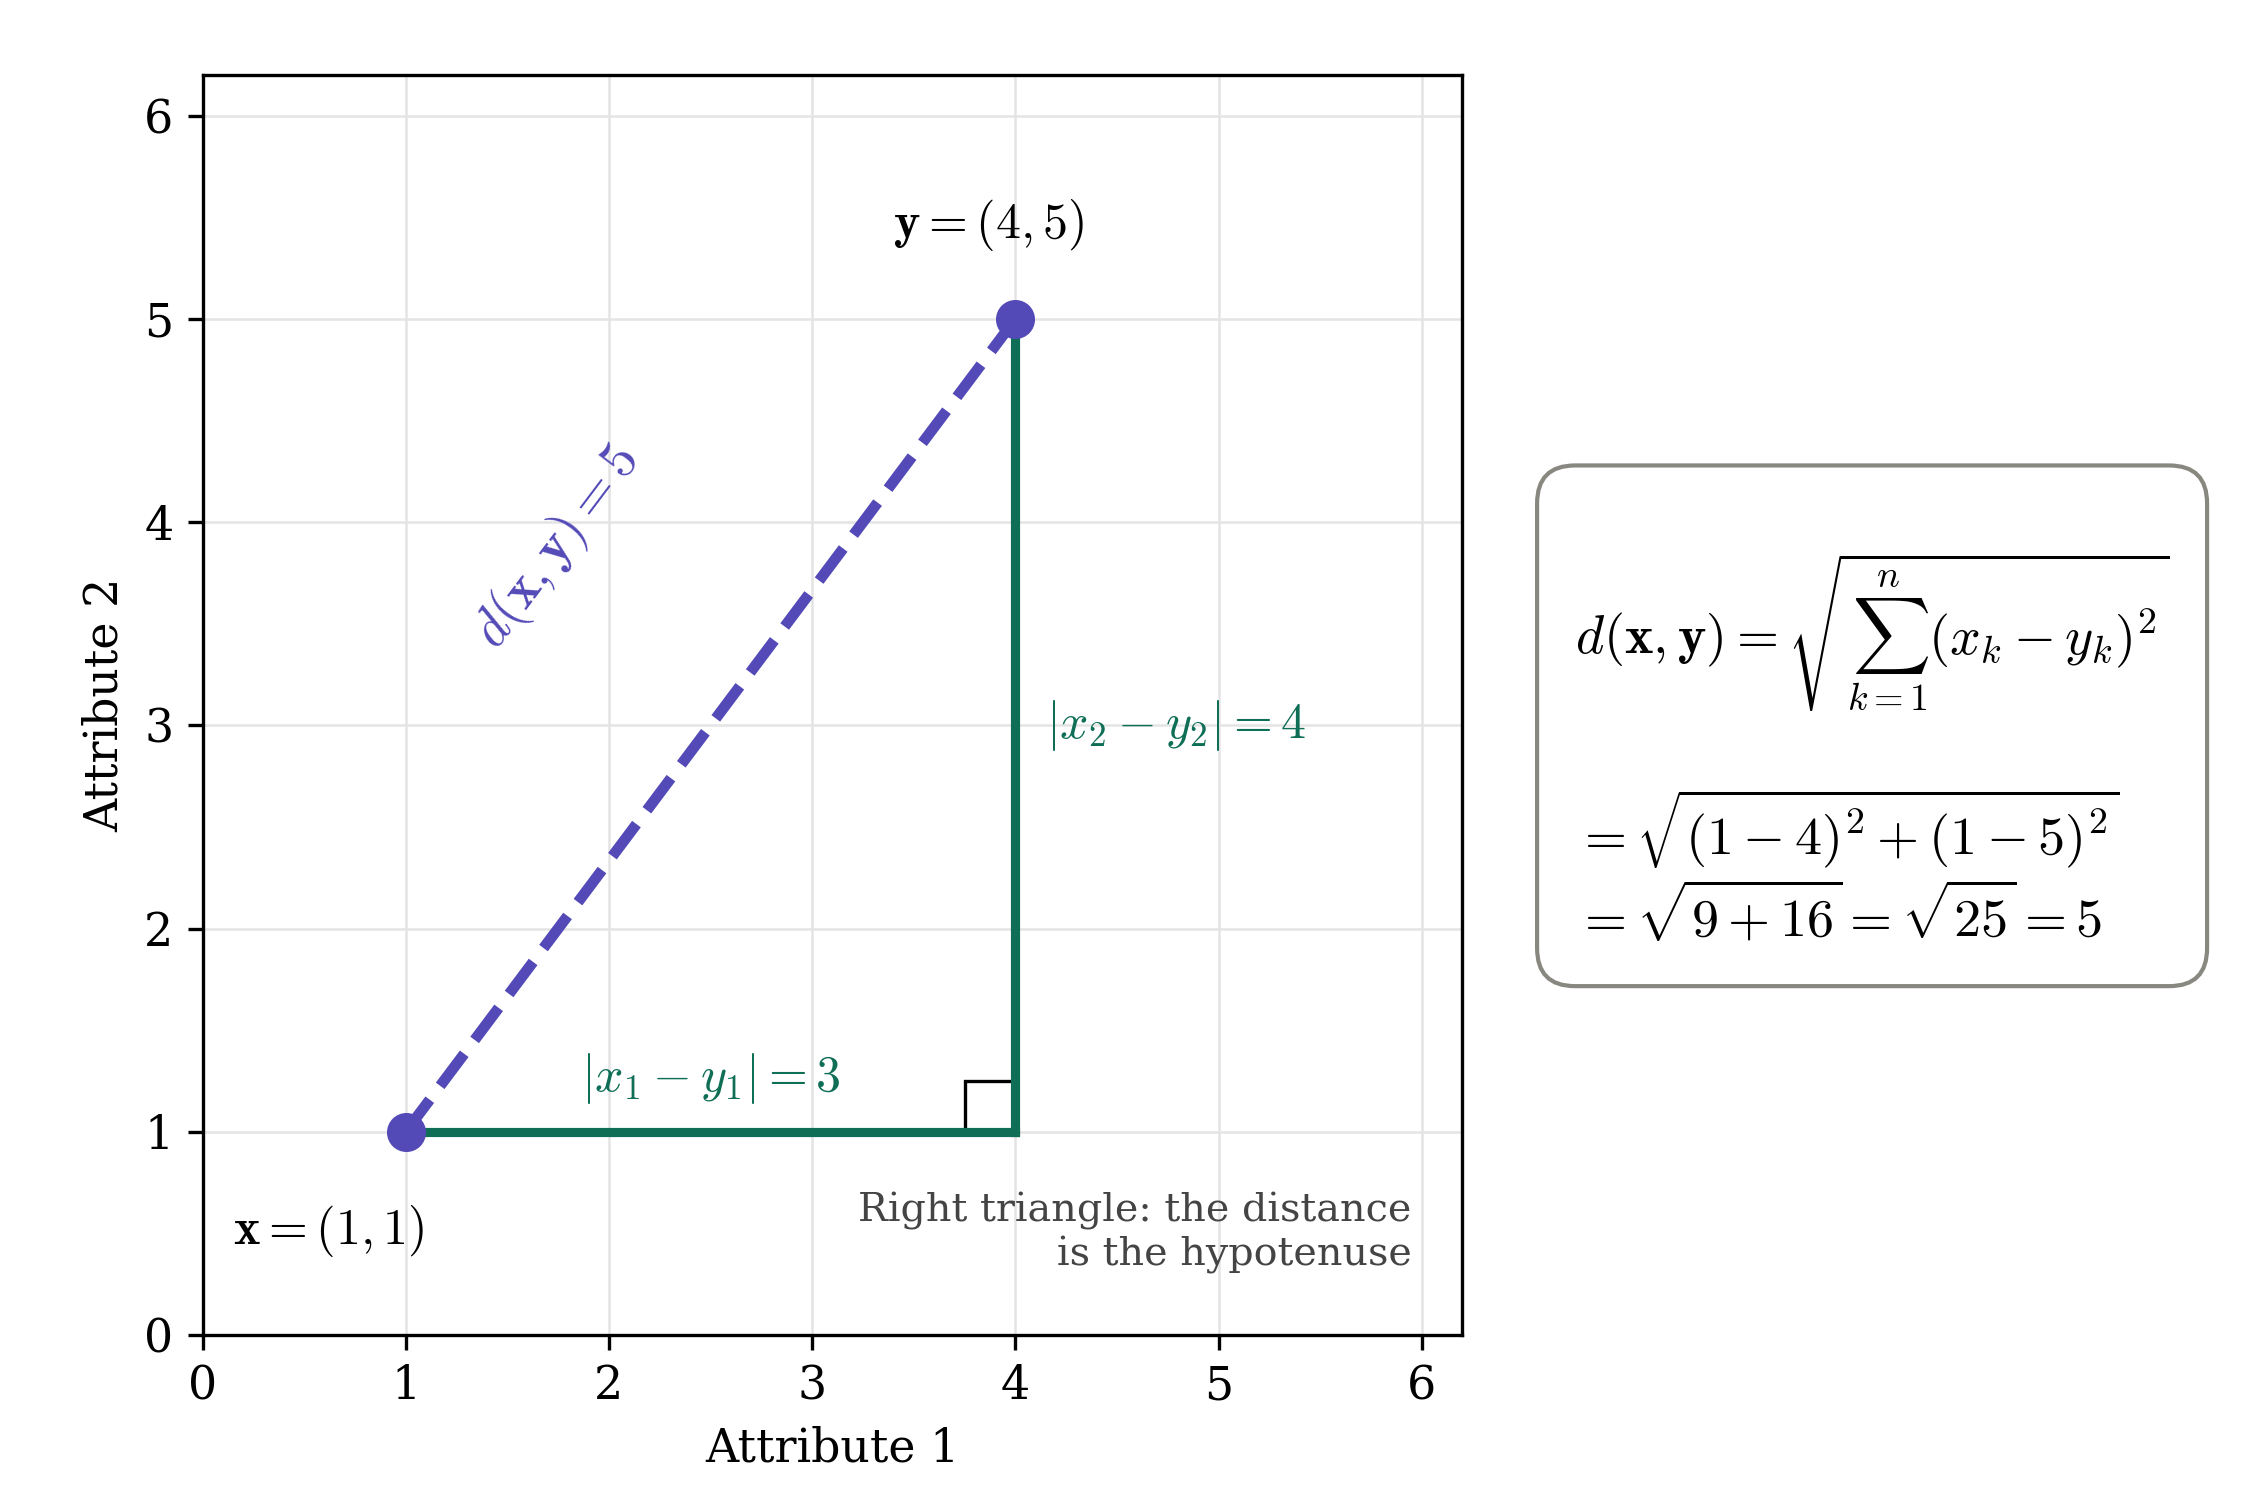
\includegraphics[width=0.5\textwidth]{images/chapter_3/euclidean_distance.png}
    \caption{Euclidean distance between $\mathbf{x}=(1,1)$ and $\mathbf{y}=(4,5)$: the per-attribute differences are the legs of a right triangle and the distance is its hypotenuse.}
\end{figure}

\begin{figure}[h]
    \centering
    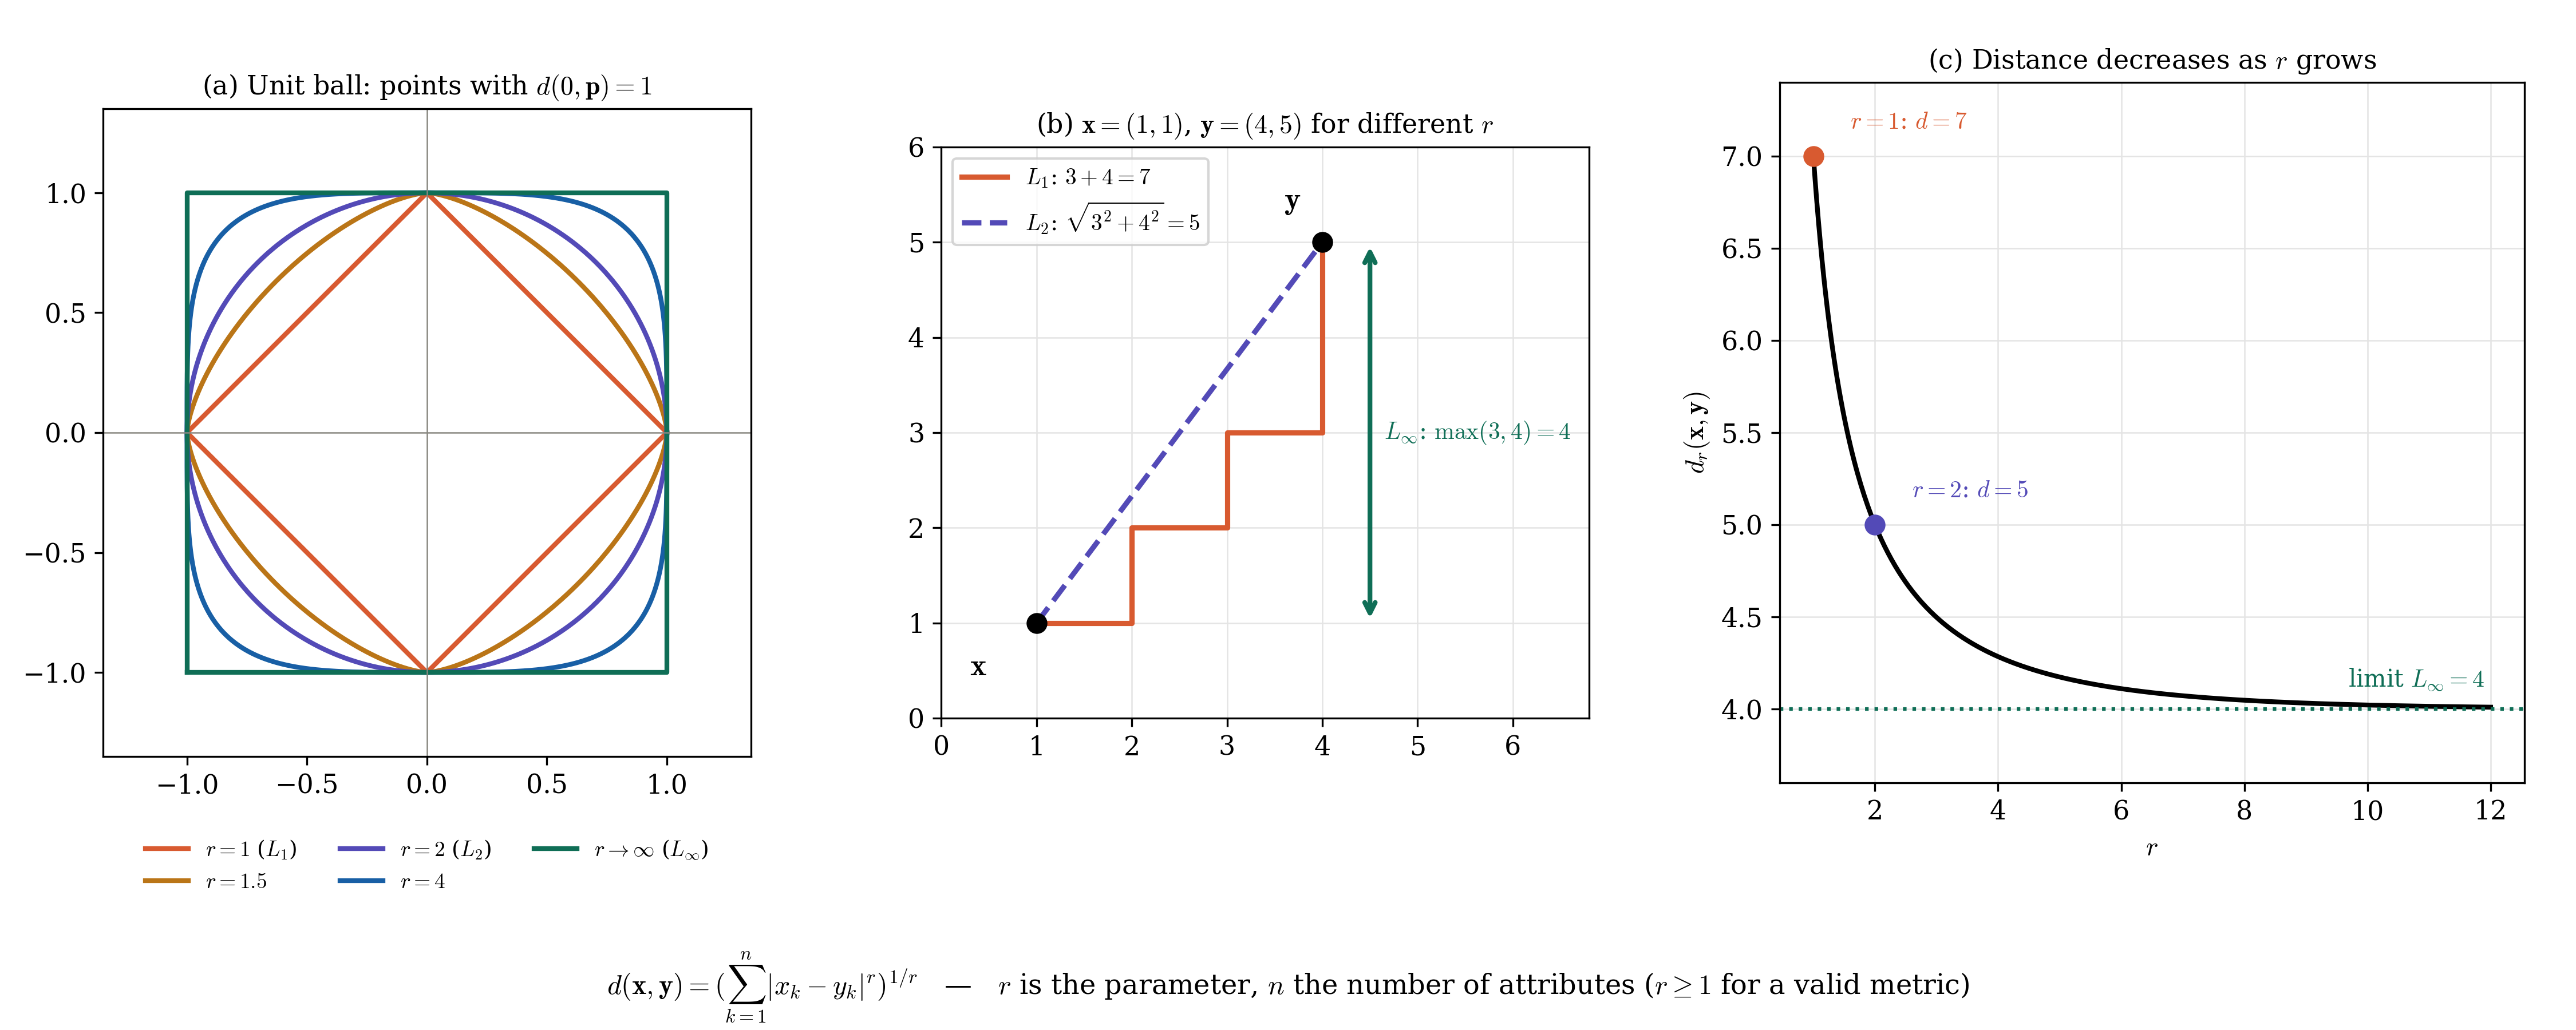
\includegraphics[width=0.5\textwidth]{images/chapter_3/minkowski_distance.png}
    \caption{Minkowski distance. (a) Unit ball for different values of $r$: a diamond for $L_1$, a circle for $L_2$, a square for $L_\infty$. (b) Distance between $\mathbf{x}=(1,1)$ and $\mathbf{y}=(4,5)$: $L_1=7$ (sum of differences), $L_2=5$ (straight line), $L_\infty=4$ (maximum difference). (c) The distance decreases as $r$ grows and converges to $L_\infty$.}
\end{figure}

\noindent\textbf{Note:} if attributes have very different scales (e.g.\ income in euros and age in years), the attribute with the largest range dominates the distance. For this reason, attributes are usually standardized before computing these distances.

\subsection{Properties of a Distance Metric}
A distance $d$ is called a \textbf{metric} if it satisfies the following properties for all points $x, y, z$ of the space:
\begin{itemize}
    \item \textbf{Identity:} the distance from a point to itself is zero: $d(x,x)=0$.
    \item \textbf{Positivity:} the distance between two distinct points is strictly positive: if $x\neq y$, then $d(x,y)>0$. Together with identity, this means that $d(x,y)=0$ if and only if $x=y$.
    \item \textbf{Symmetry:} the order of the points does not matter: $d(x,y)=d(y,x)$.
    \item \textbf{Triangle Inequality:} going directly from $x$ to $z$ is never longer than passing through an intermediate point $y$: $d(x,z)\le d(x,y)+d(y,z)$.
\end{itemize}

\begin{figure}[h]
    \centering
    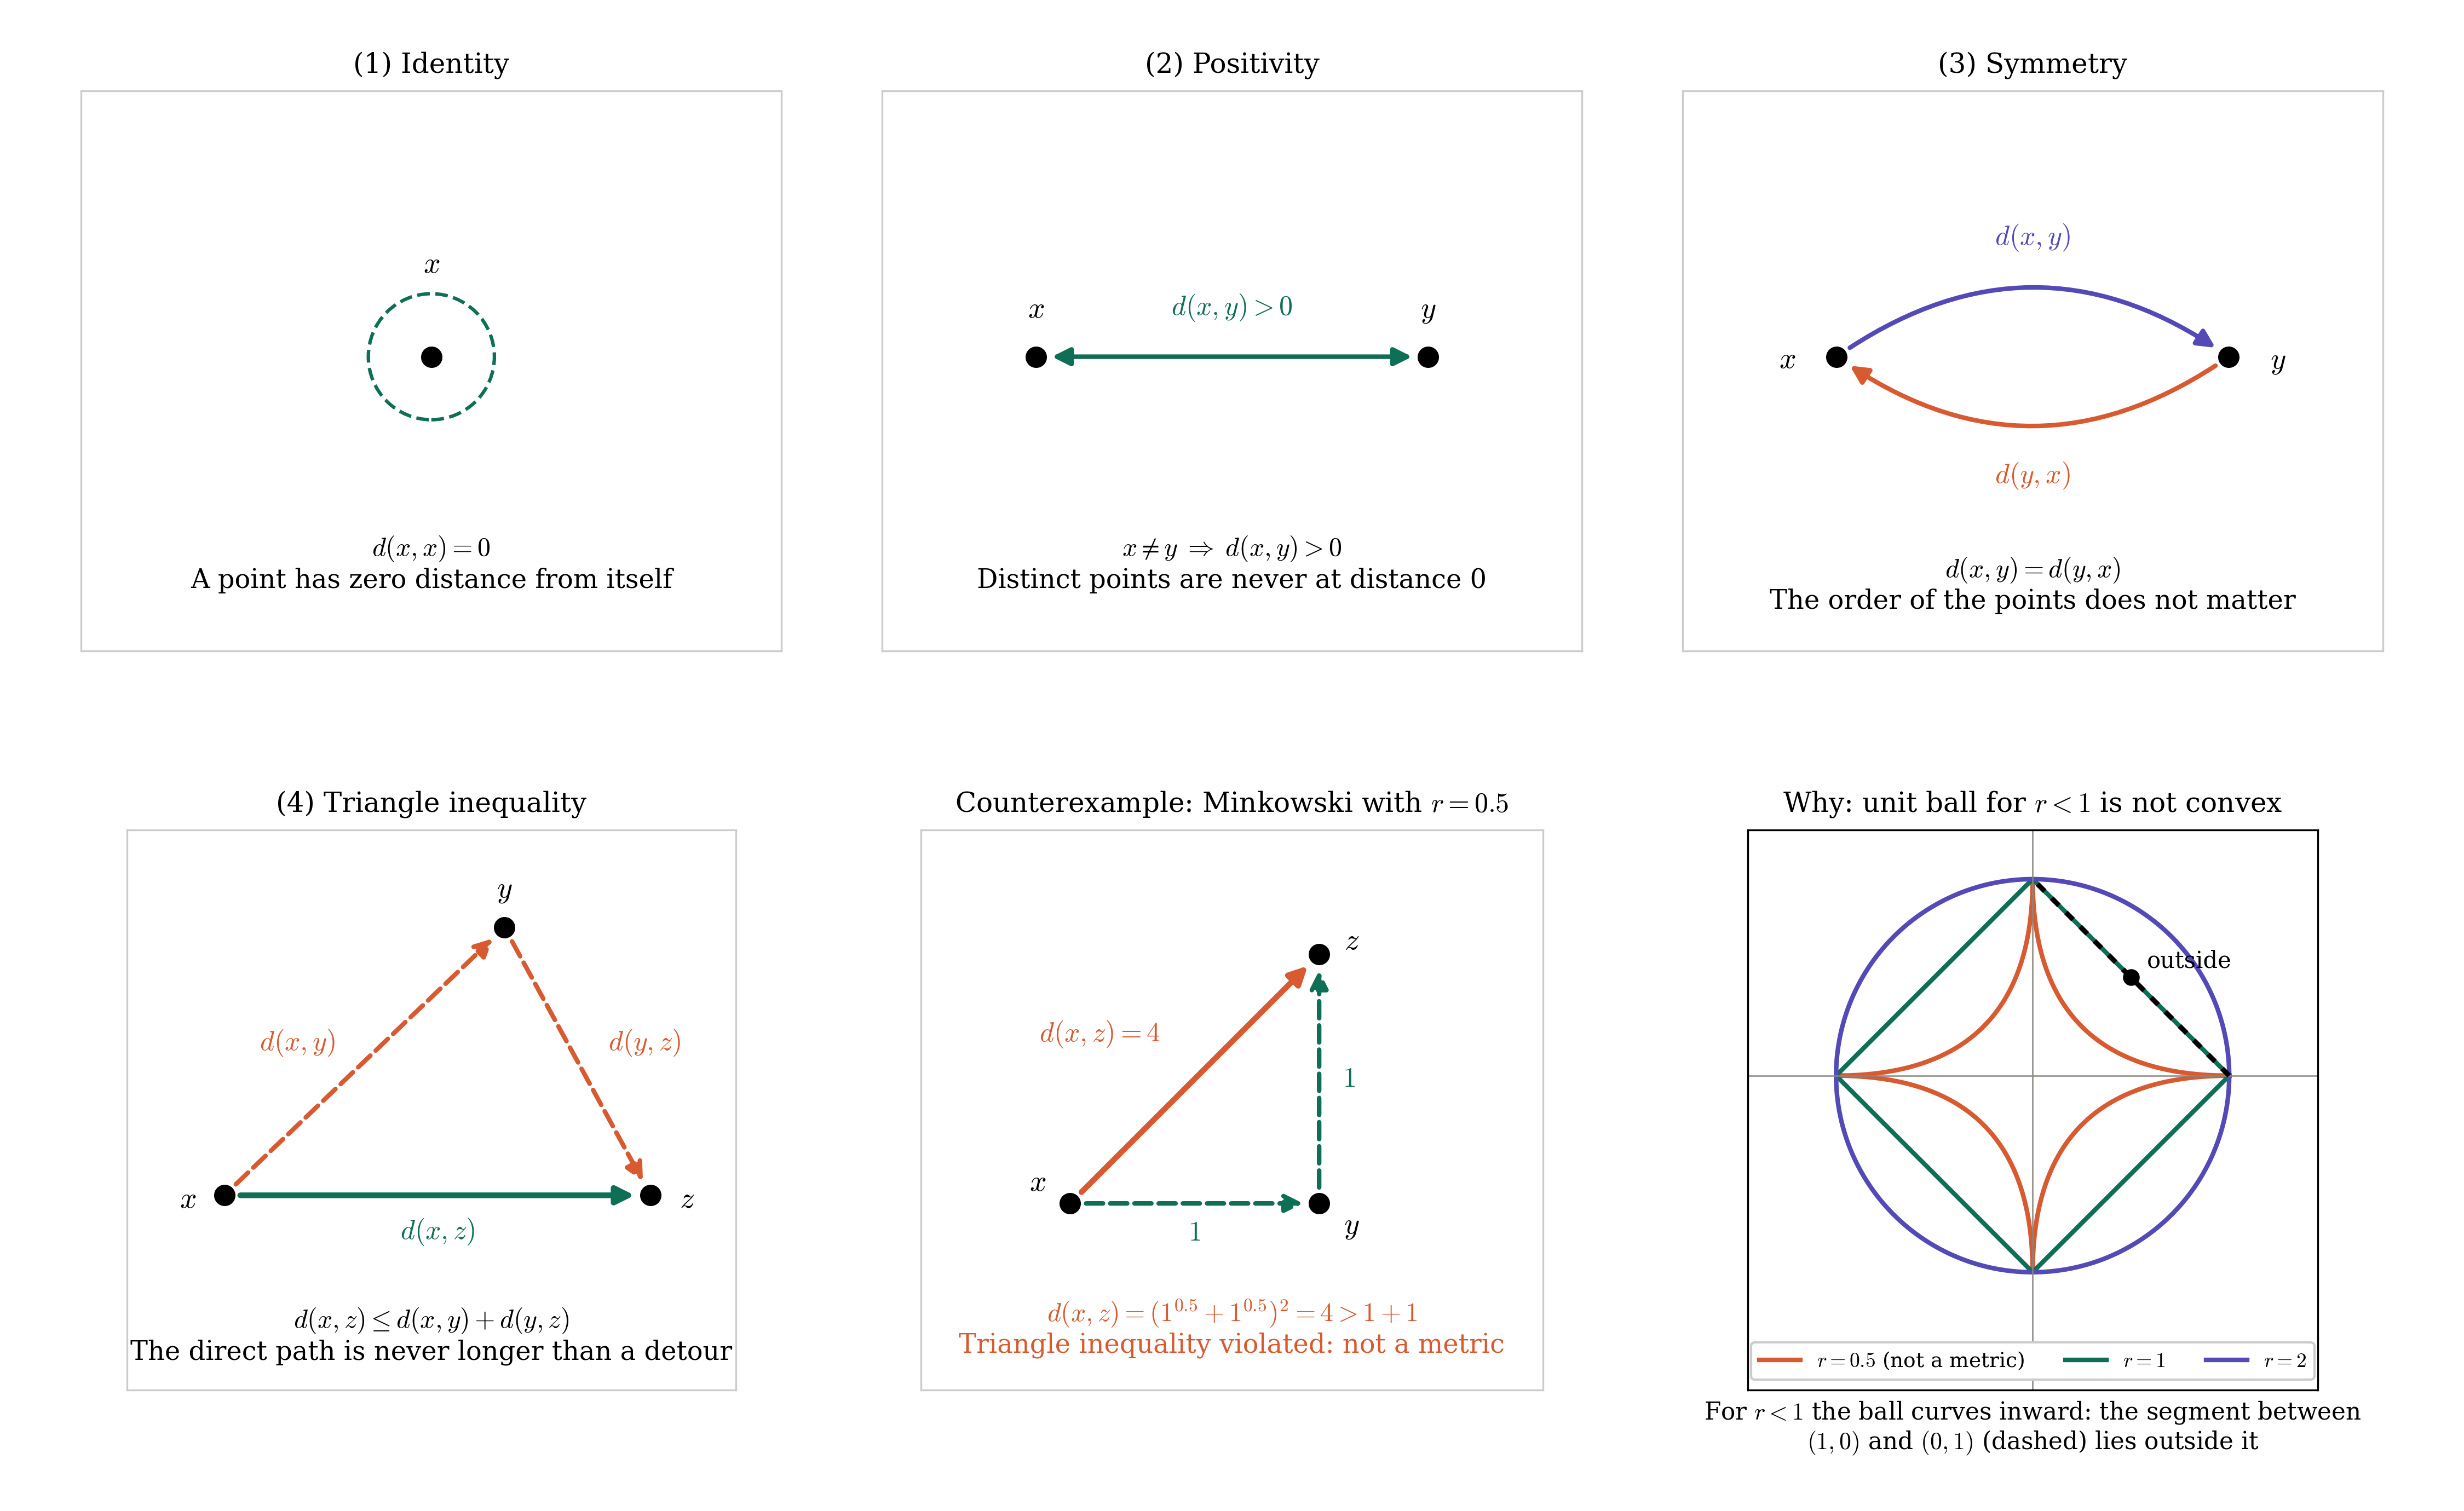
\includegraphics[width=0.8\textwidth]{images/chapter_3/distance_metric_properties.png}
    \caption{Properties of a distance metric. (1)--(4) The four properties: identity, positivity, symmetry and triangle inequality. Bottom centre: the Minkowski distance with $r=0.5$ violates the triangle inequality, since $d(x,z)=4>d(x,y)+d(y,z)=2$. Bottom right: for $r<1$ the unit ball is not convex, which is the geometric reason why the triangle inequality fails.}
\end{figure}

The Minkowski distance is a metric for every $r\geq1$. For $r<1$ the triangle inequality is violated: for instance, with $r=0.5$, $x=(0,0)$, $z=(1,1)$ and $y=(1,0)$ we get $d(x,z)=(1+1)^2=4$, while $d(x,y)+d(y,z)=1+1=2$, so the direct path would be longer than the detour.

\subsection{Mahalanobis Distance}
The Mahalanobis distance measures the distance between two points while taking into account the distribution of the data, described by its covariance matrix $S$:
\[
    d(\mathbf{x},\mathbf{y};S)=\sqrt{(\mathbf{x}-\mathbf{y})^\top S^{-1}(\mathbf{x}-\mathbf{y})}
\]
The inverse covariance matrix $S^{-1}$ reweights the differences between the points:

\begin{itemize}
    \item along directions where the data have \textbf{high variance}, a difference counts \emph{less}, because large spreads are normal there;
    \item along directions where the data have \textbf{low variance}, the same difference counts \emph{more}, because it is unusual;
    \item \textbf{correlations} between attributes are also taken into account, so redundant information is not counted twice.
\end{itemize}

As a consequence, the Mahalanobis distance is unitless and scale-invariant. Two special cases help to interpret it:

\begin{figure}[h]
    \centering
    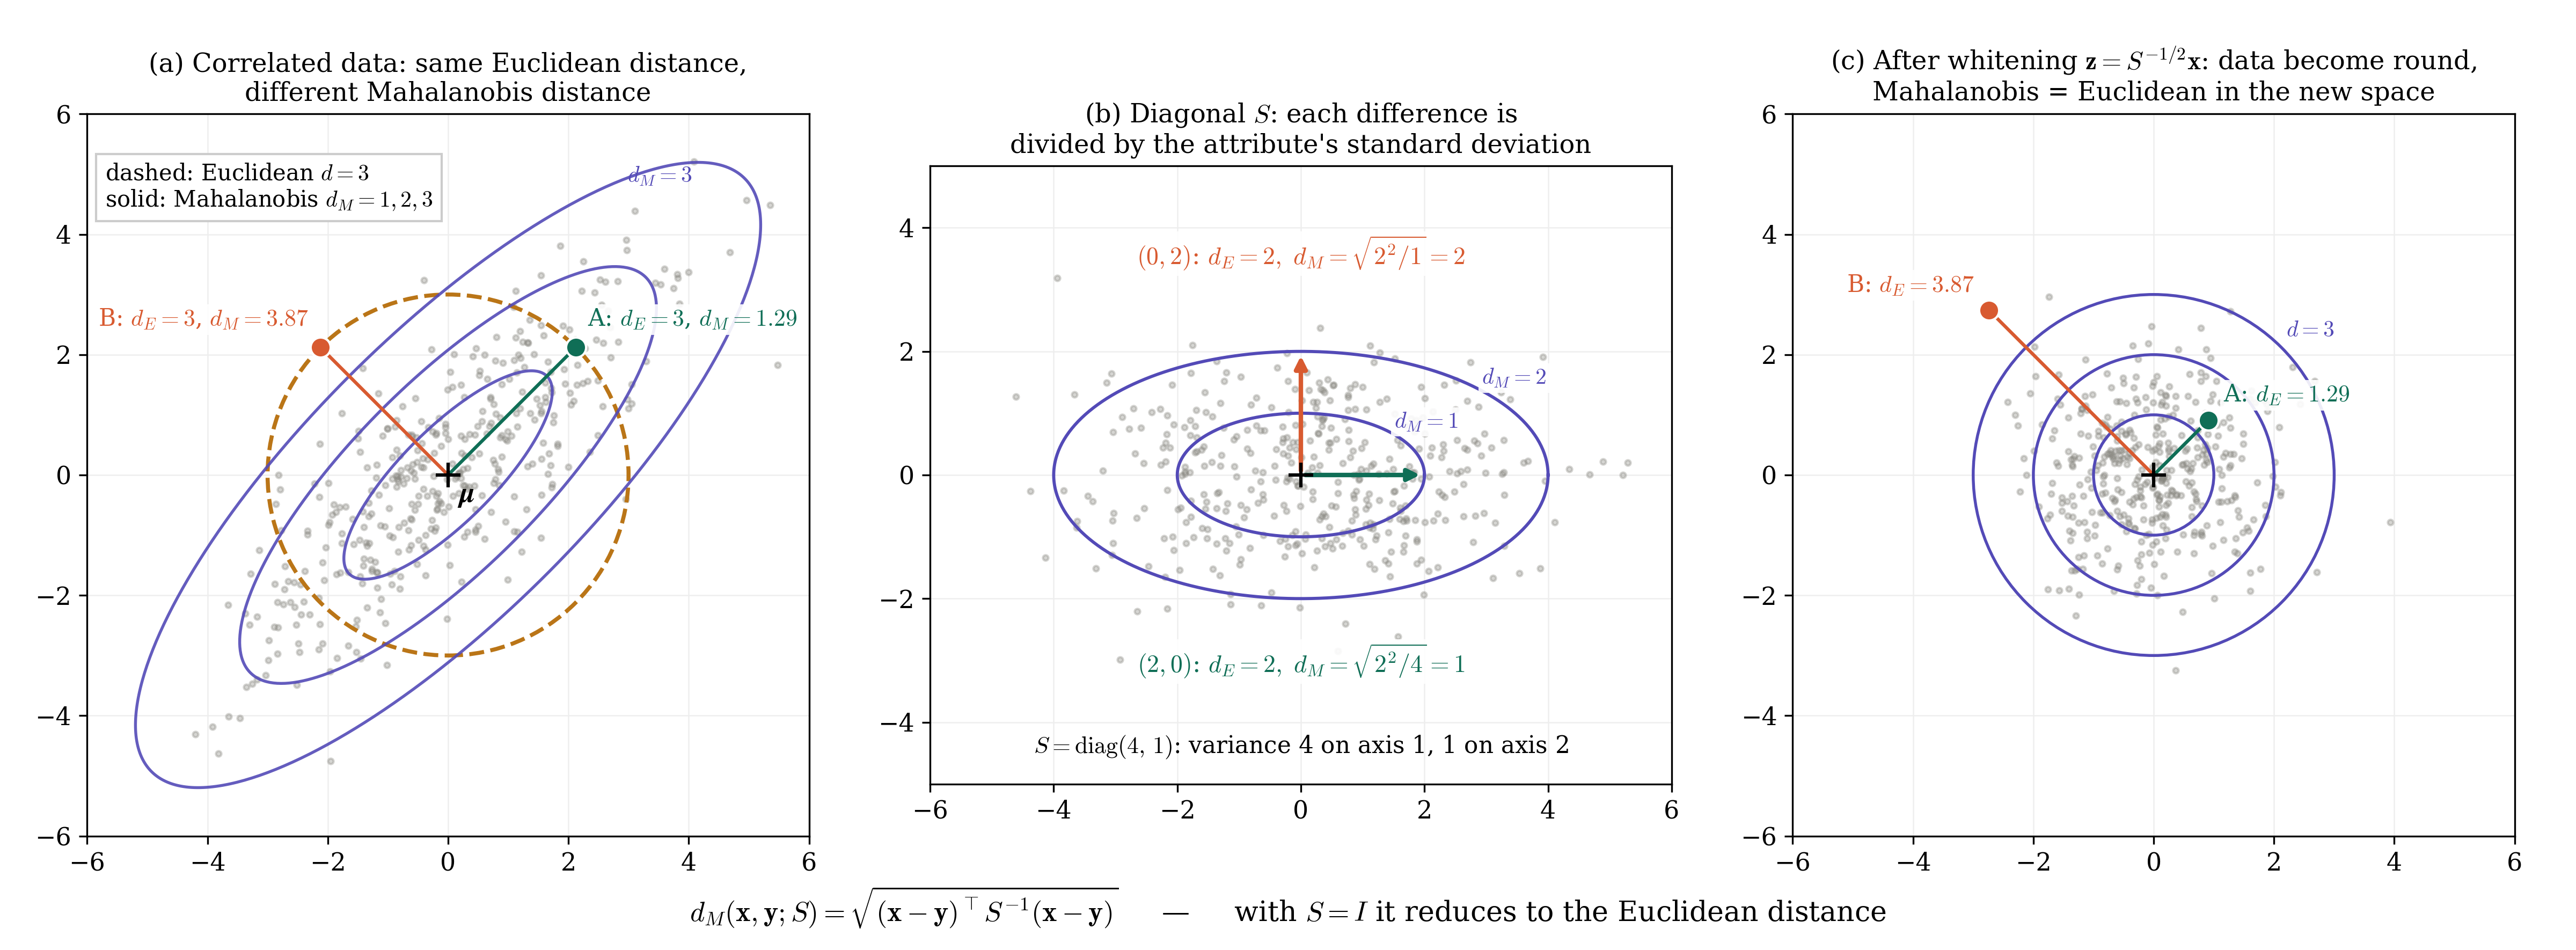
\includegraphics[width=0.8\textwidth]{images/chapter_3/mahalanobis_distance.png}
    \caption{Mahalanobis distance. (a) With correlated data, points A and B have the same Euclidean distance from the mean $\boldsymbol{\mu}$, but A lies along the direction of high variance ($d_M=1.29$) while B lies across it ($d_M=3.87$): the contours of constant Mahalanobis distance are ellipses that follow the shape of the data. (b) With a diagonal $S$ each difference is divided by the standard deviation of its attribute: the same Euclidean difference of $2$ gives $d_M=1$ along the high-variance axis and $d_M=2$ along the low-variance one. (c) Transforming the data with $S^{-1/2}$ (whitening) makes the distribution round, and the Euclidean distance in the new space equals the Mahalanobis distance in the original one.}
\end{figure}

\begin{itemize}
    \item if $S=I$ (identity matrix: unit variances and no correlation), it reduces to the \textbf{Euclidean distance};
    \item if $S$ is diagonal, it is equivalent to the Euclidean distance computed on \textbf{standardized} attributes, i.e.\ each difference is divided by the standard deviation of its attribute.
\end{itemize}
\textbf{Example:} let $S=\begin{pmatrix}4&0\\0&1\end{pmatrix}$, so the first attribute has variance $4$ and the second variance $1$. For a difference $\mathbf{x}-\mathbf{y}=(2,0)$ we get $d=\sqrt{2^2/4}=1$, while for $\mathbf{x}-\mathbf{y}=(0,2)$ we get $d=\sqrt{2^2/1}=2$. Both pairs have Euclidean distance $2$, but the Mahalanobis distance considers the second pair farther apart, since a difference of $2$ is much less common along the second attribute.

\section{Data PreProcessing}
Real-world data are rarely ready to be analysed: they can be noisy, redundant, too large, described by too many attributes, or stored in formats that algorithms cannot handle (e.g.\ text). \textbf{Data PreProcessing} is the set of techniques that turn raw data into a form that is cleaner, smaller and more suitable for the analysis. The main techniques are:
\begin{itemize}
    \item \textbf{Data Aggregation:} combining two or more attributes or objects into a single one.
    \item \textbf{Data Reduction:} obtaining a smaller dataset that gives (almost) the same analytical results.
    \item \textbf{Feature Selection:} keeping only the useful attributes, needed to tackle the \emph{curse of dimensionality} (Section~\ref{sec:curse}).
    \item \textbf{Feature Transformation or Normalization:} changing the values or the scale of attributes (Sections~\ref{sec:transformation}--\ref{sec:attr-transformation}).
    \item \textbf{Preprocessing for textual data:} turning documents into structured data (Section~\ref{sec:documents}).
\end{itemize}

\paragraph{Data Aggregation.} Aggregation replaces a group of objects (or attributes) with a single one that summarises them, typically with a sum or an average. Examples: daily sales $\rightarrow$ monthly sales, cities $\rightarrow$ regions, single transactions $\rightarrow$ total per customer. It is used for three purposes:
\begin{itemize}
    \item \textbf{data reduction:} fewer objects to store and process (365 days become 12 months);
    \item \textbf{change of scale:} looking at the data at a coarser level of detail (regions instead of cities);
    \item \textbf{more stable data:} averages vary less than single values, because random fluctuations tend to cancel out (Figure~\ref{fig:aggregation}).
\end{itemize}
The price to pay is the loss of detail: after aggregating into months, it is no longer possible to know what happened on a specific day.

\begin{figure}[htbp]
    \centering
    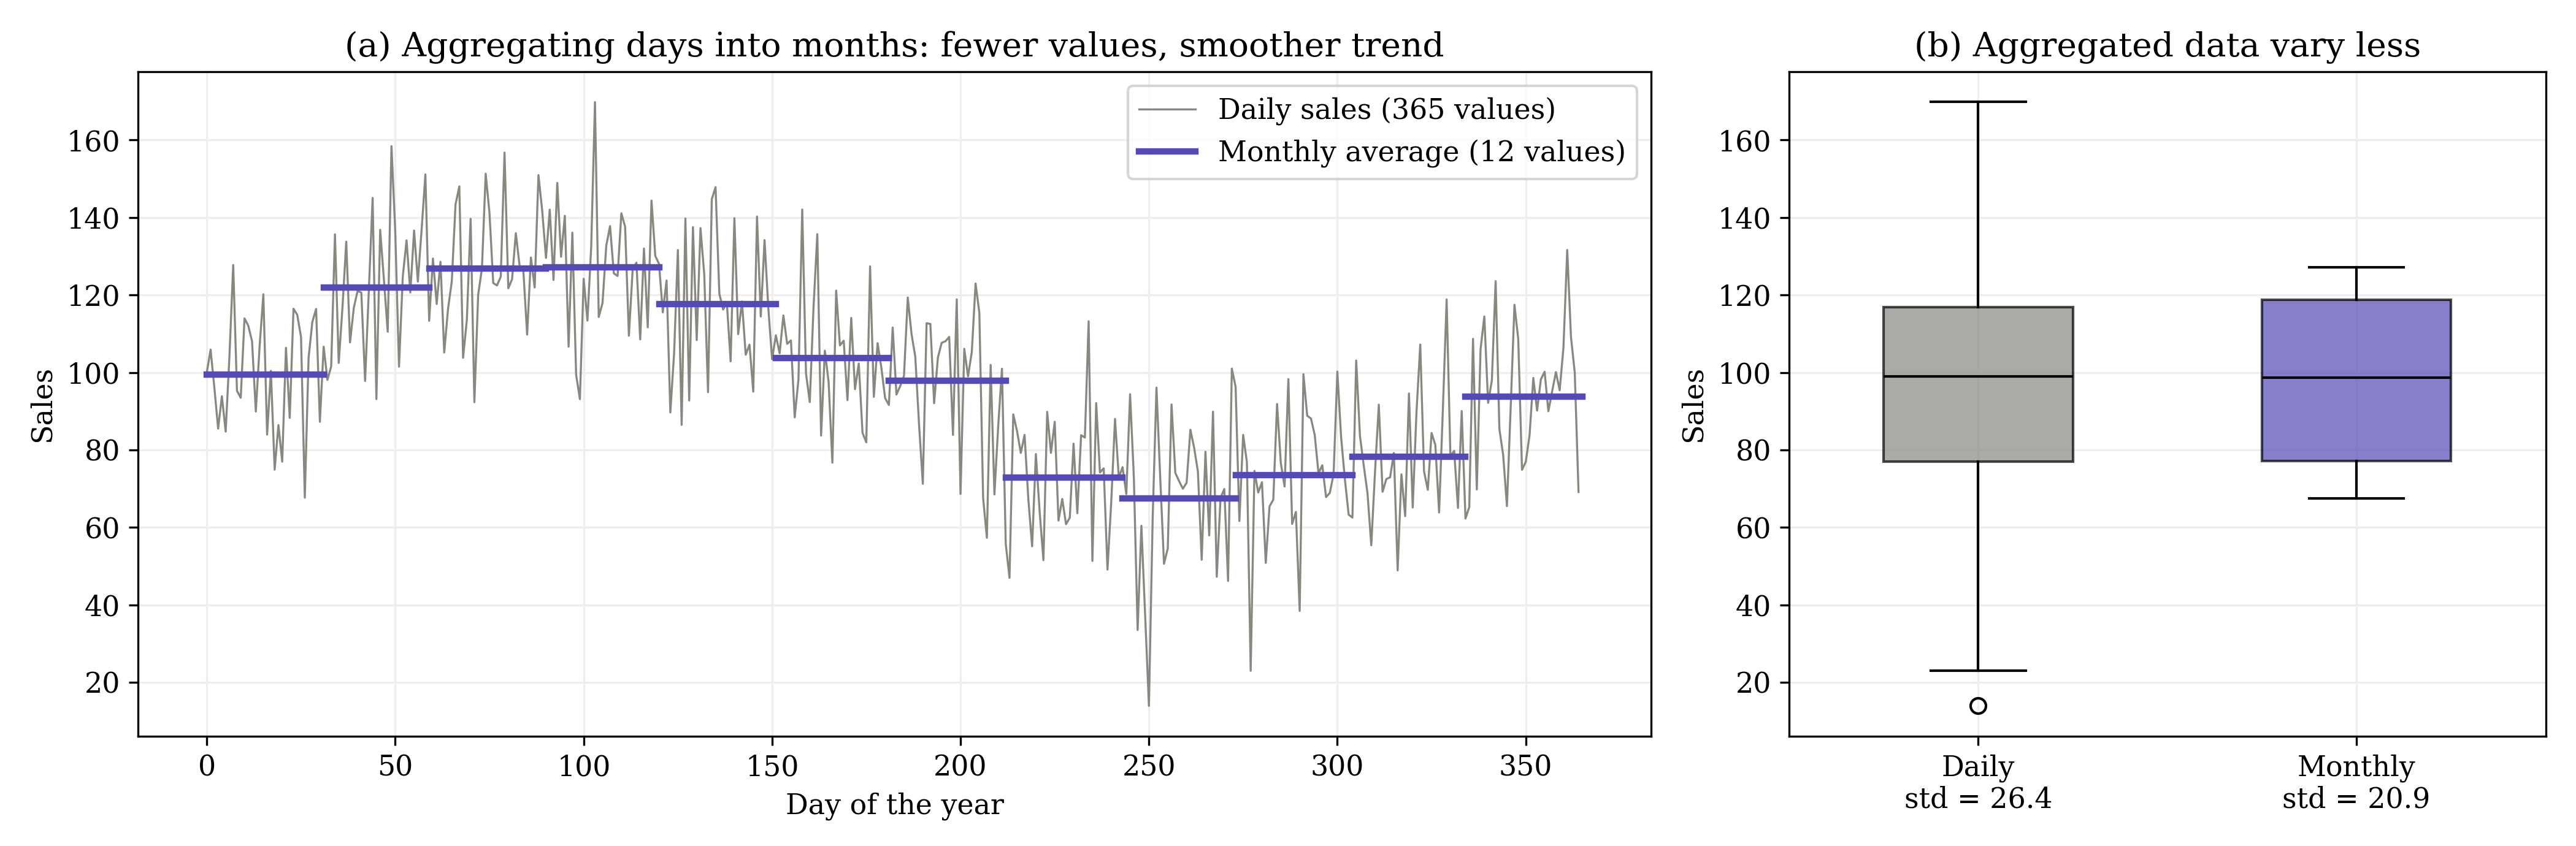
\includegraphics[width=0.8\textwidth]{images/chapter_3/aggregation.png}
    \caption{Data aggregation. (a) 365 daily values are replaced by 12 monthly averages, which show the trend more clearly. (b) The aggregated values have a lower variability (smaller standard deviation) than the original ones.}
\end{figure}

\paragraph{Data Reduction.} Data reduction generates a reduced representation of the dataset, \emph{smaller in volume but able to provide similar analytical results}. A dataset is a table, so it can be reduced along three directions:
\begin{itemize}
    \item \textbf{fewer rows}, i.e.\ fewer objects: \emph{sampling} (reduces the cardinality of the dataset);
    \item \textbf{fewer columns}, i.e.\ fewer attributes: \emph{feature selection and creation};
    \item \textbf{fewer distinct values per column}: \emph{discretization} (reduces the cardinality of the attribute domains, e.g.\ age $\rightarrow$ \{young, adult, senior\}).
\end{itemize}

\paragraph{Sampling.} Sampling is the main technique for data selection and reduction: instead of analysing all the objects, only a subset of them (the \emph{sample}) is analysed. It is useful when processing the whole dataset is too expensive or too slow. It is based on two key principles:
\begin{itemize}
    \item using a sample works almost as well as using the entire dataset, \emph{if the sample is representative};
    \item a sample is \textbf{representative} if it has approximately the same property of interest as the original dataset (e.g.\ the same mean, or the same proportion of each class).
\end{itemize}
There are two main types of sampling:
\begin{itemize}
    \item \textbf{Simple Random Sampling:} every object has the same probability of being selected. It is simple, but with small samples or rare classes it may produce an unrepresentative sample by chance: a class that is $10\%$ of the data could be missing entirely (Figure~\ref{fig:sampling}b).
    \item \textbf{Stratified Sampling:} the data are first split into groups (\emph{strata}), for instance one per class, and then a random sample is drawn from each group, proportionally to its size. This guarantees that every group is represented with the right proportion (Figure~\ref{fig:sampling}c).
\end{itemize}

\begin{figure}[htbp]
    \centering
    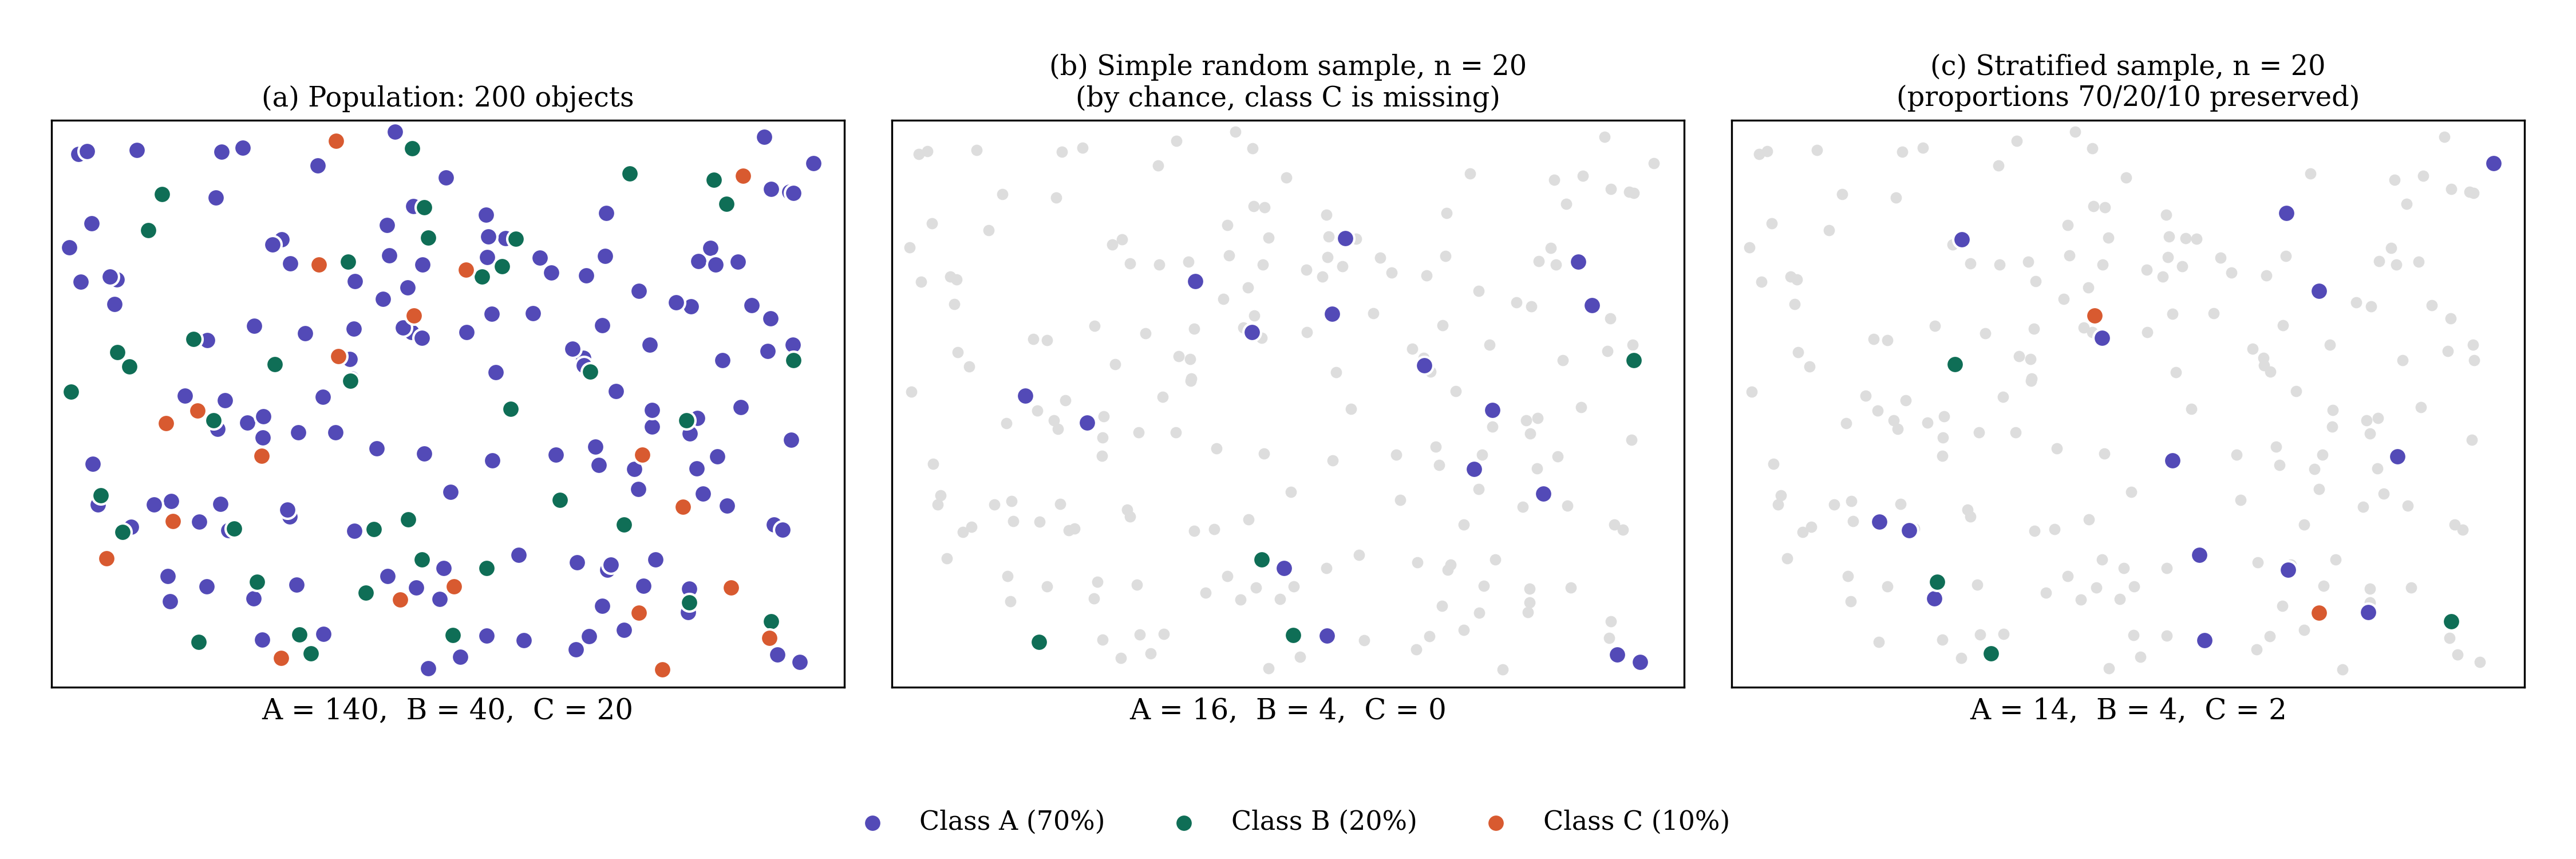
\includegraphics[width=0.8\textwidth]{images/chapter_3/sampling.png}
    \caption{Sampling 20 objects from a population of 200 with imbalanced classes (70\%, 20\%, 10\%). Simple random sampling may miss the rarest class, while stratified sampling preserves the original proportions.}
\end{figure}

\subsection{Curse of Dimensionality}
The \textbf{curse of dimensionality} is the set of problems that arise when the number of attributes (dimensions) becomes large. The key idea is simple: \emph{when the number of dimensions increases, the volume of the space grows so fast that the data become sparse}, i.e.\ points are far from each other and the space is mostly empty.

Two effects make this concrete (Figure~\ref{fig:curse}):
\begin{itemize}
    \item \textbf{Neighbourhoods are no longer local.} With uniform data in a unit cube, a sub-cube that contains $10\%$ of the points has edge $0.1$ in 1 dimension, but edge $0.79$ in 10 dimensions: to find ``nearby'' points one must cover almost the whole range of every attribute.
    \item \textbf{Distances become all similar.} As the dimensions grow, the distance to the nearest point and the distance to the farthest point become almost the same. If all points are roughly equally distant, the concept of ``near'' loses its meaning.
\end{itemize}
As a consequence, the definitions of \textbf{density} and \textbf{distance} between points, which are critical for clustering and outlier detection, become less meaningful.

\begin{figure}[htbp]
    \centering
    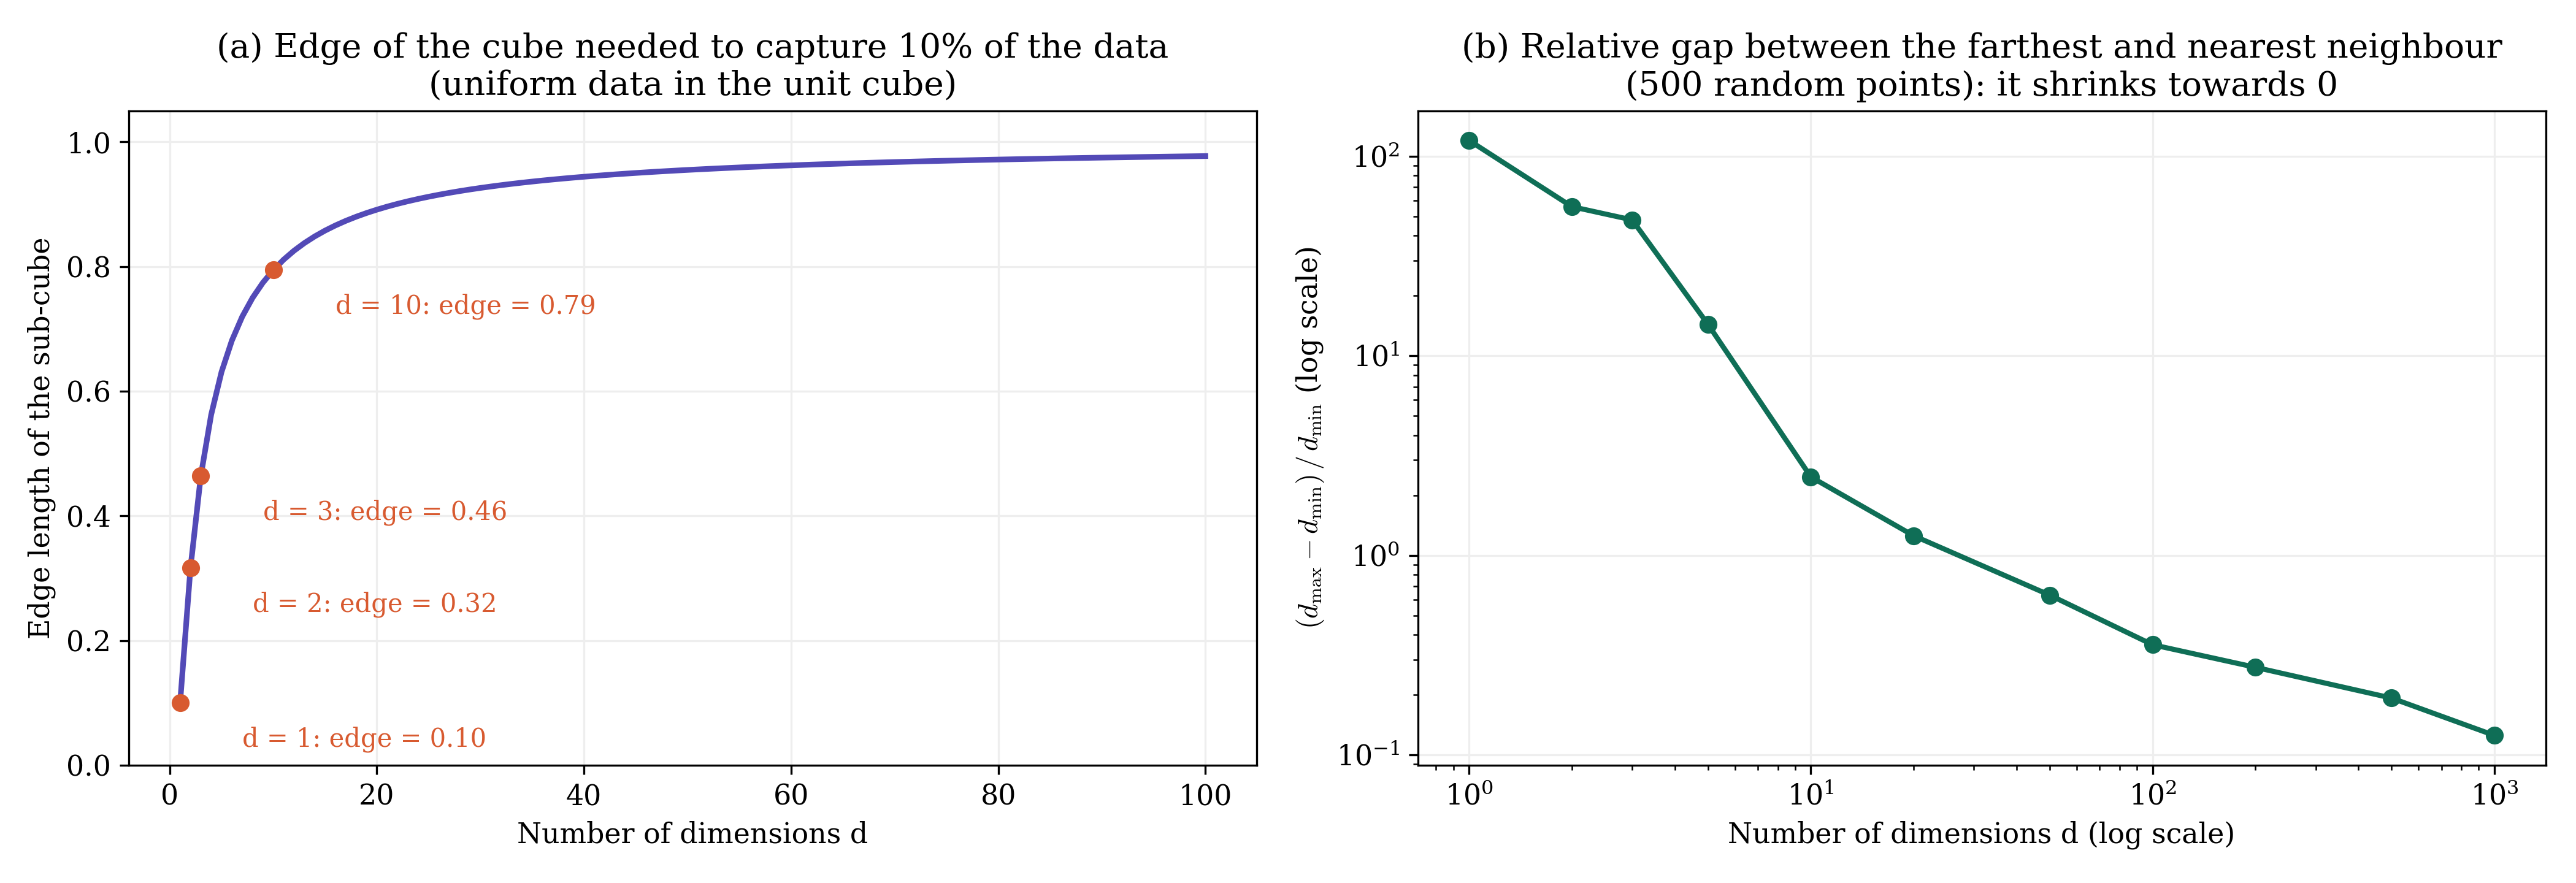
\includegraphics[width=0.8\textwidth]{images/chapter_3/curse_of_dimensionality.png}
    \caption{Curse of dimensionality. (a) To capture 10\% of uniformly distributed data, the edge of the sub-cube quickly approaches the full range as the number of dimensions grows. (b) The relative difference between the farthest and the nearest neighbour shrinks towards zero: in high dimensions all points look equally distant.}
\end{figure}

\paragraph{Feature Subset Selection.} One way to counter the curse of dimensionality is to keep only a subset of the attributes. Feature Subset Selection reduces the dimensionality of the data by removing:
\begin{itemize}
    \item \textbf{redundant features}, which duplicate much or all of the information contained in other attributes. Example: the price of a product with and without VAT; knowing one, the other adds nothing.
    \item \textbf{irrelevant features}, which contain no useful information for the task at hand. Example: the student ID when predicting the student's grade.
\end{itemize}

\paragraph{Recursive Feature Elimination (RFE).} A common way to perform feature selection is to remove features one step at a time, always discarding the least useful one (Figure~\ref{fig:rfe}):
\begin{enumerate}
    \item assign a weight (importance) to each feature, for instance the absolute value of the coefficients of a linear model;
    \item train the model (\emph{estimator}) on the current set of features and obtain the importance of each feature;
    \item remove (\emph{prune}) the least important feature(s) from the current set;
    \item repeat steps 2--3 on the reduced set, until the desired number of features is reached.
\end{enumerate}
The model is retrained at every iteration because removing a feature can change the importance of the others. For the same reason, RFE can be expensive when there are many features.

\begin{figure}[htbp]
    \centering
    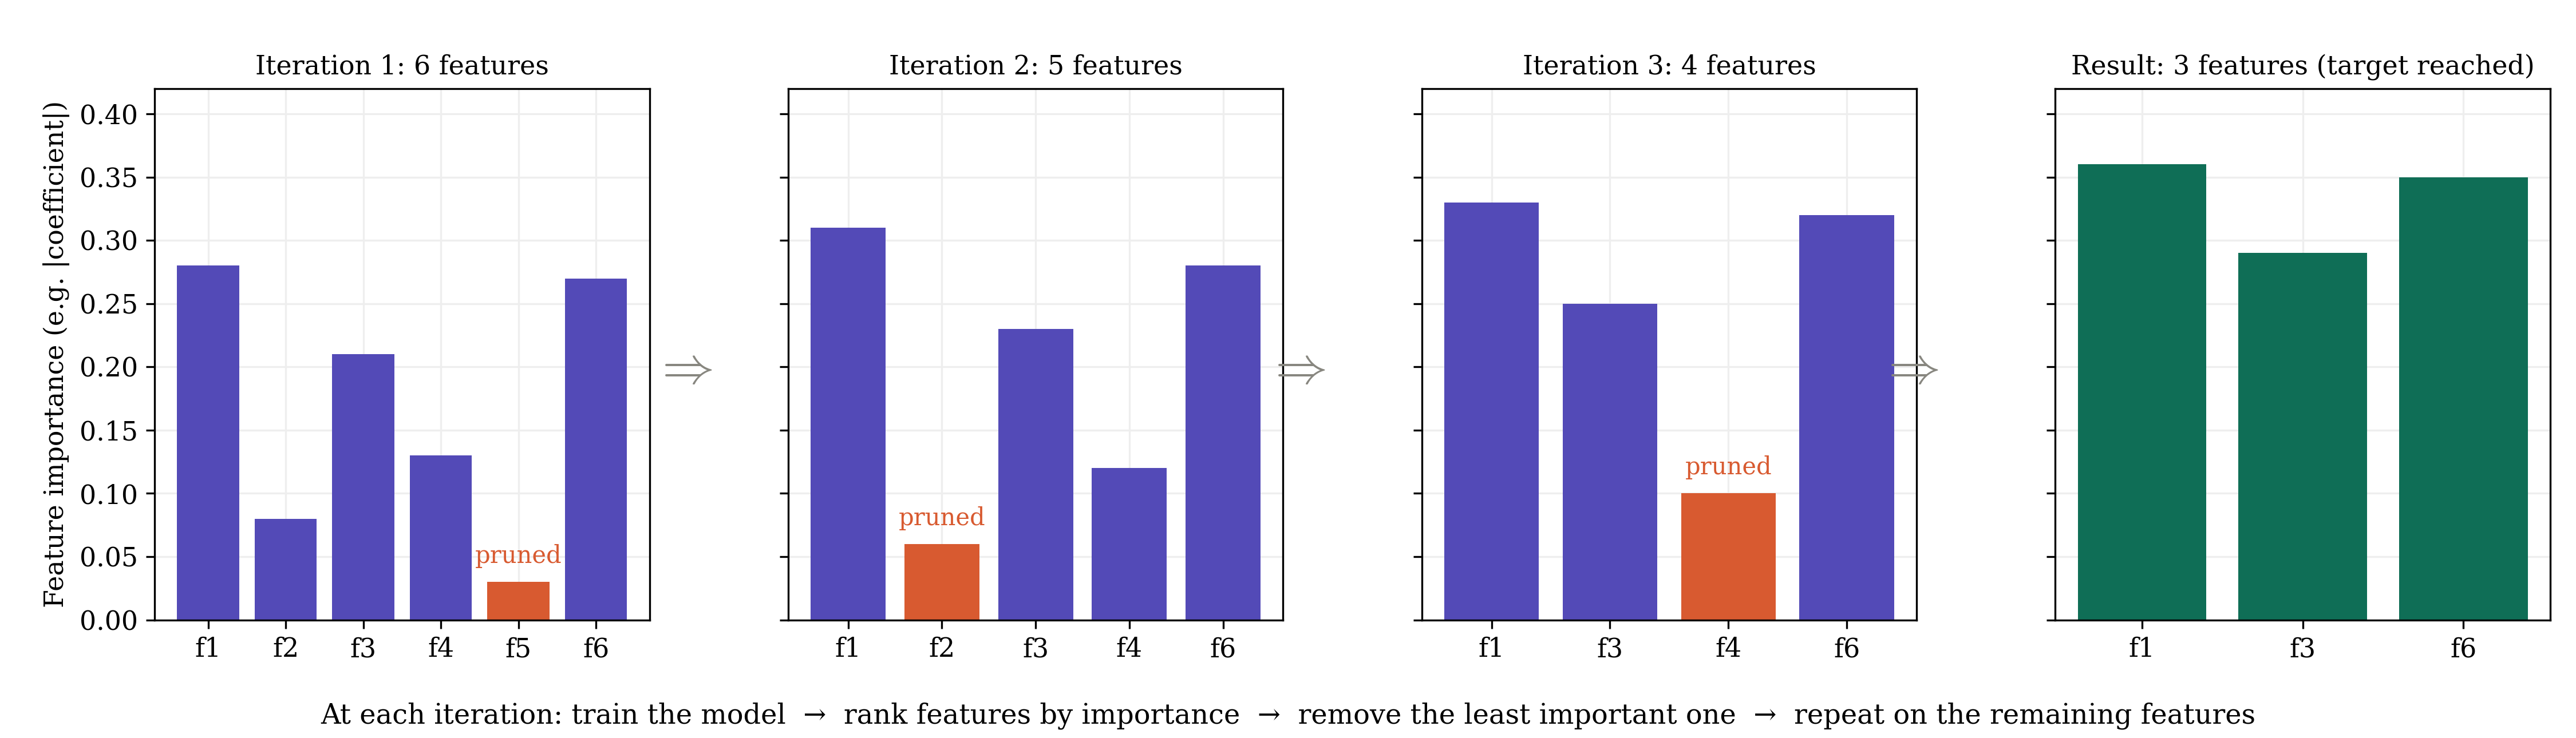
\includegraphics[width=0.8\textwidth]{images/chapter_3/rfe.png}
    \caption{Recursive Feature Elimination with a target of 3 features. At each iteration the model is retrained, the importances are recomputed and the least important feature (in orange) is removed.}
\end{figure}

\paragraph{Other approaches.}
\begin{itemize}
    \item \textbf{Feature importance of interpretable models:} some models directly tell how much each feature contributes to the prediction, for instance Decision Trees (how much each feature is used to split the data) and Linear Regression (the size of the coefficients, if the features are on the same scale). The least important features can then be discarded.
    \item \textbf{Decomposition techniques} such as PCA and SVD can be used to reduce dimensionality automatically. Strictly speaking, they do not select original features but \emph{create new ones}: each component is a combination of the original attributes, and the first few components capture most of the information in the data. Looking at how much each original attribute contributes to the main components also tells which attributes are the most important.
\end{itemize}

\subsection{Feature Engineering}
\textbf{Feature Engineering} is the act of extracting features from raw data and transforming them into formats that are more suitable for a Machine Learning model. A good representation of the data often matters more than the choice of the algorithm. Different techniques are needed according to the type of data:

\begin{center}
    \small
    \renewcommand{\arraystretch}{1.3}
    \begin{tabular}{|l|p{3.6cm}|p{5.2cm}|}
    \hline
    \textbf{Data type} & \textbf{Examples} & \textbf{Typical techniques} \\
    \hline
    Structured & numerical, categorical attributes & normalization, discretization, binarization (one-hot encoding) \\
    \hline
    Unstructured & text, images, signals & tokenization and term vectors, Fourier transform, extraction of descriptors \\
    \hline
    Mixed & e.g.\ a product with price, category and description & combination of the above \\
    \hline
    \end{tabular}
\end{center}

The basic Feature Engineering techniques, described in the next subsections, are \textbf{data transformation}, \textbf{discretization}, \textbf{binarization} and \textbf{normalization}.

\subsection{Data Transformation}
Data transformation is the process of converting data from one format or representation to another, so that the important information is captured much more efficiently than in the original representation.

The classic example is the \textbf{Fourier Transform}, which converts a signal from the \emph{time domain} (value at each instant) to the \emph{frequency domain} (which frequencies the signal contains, and how strong they are). A signal made of a few overlapping waves looks complicated as a sequence of values, but in the frequency domain it is summarised by a few peaks (Figure~\ref{fig:fourier}).

\begin{figure}[htbp]
    \centering
    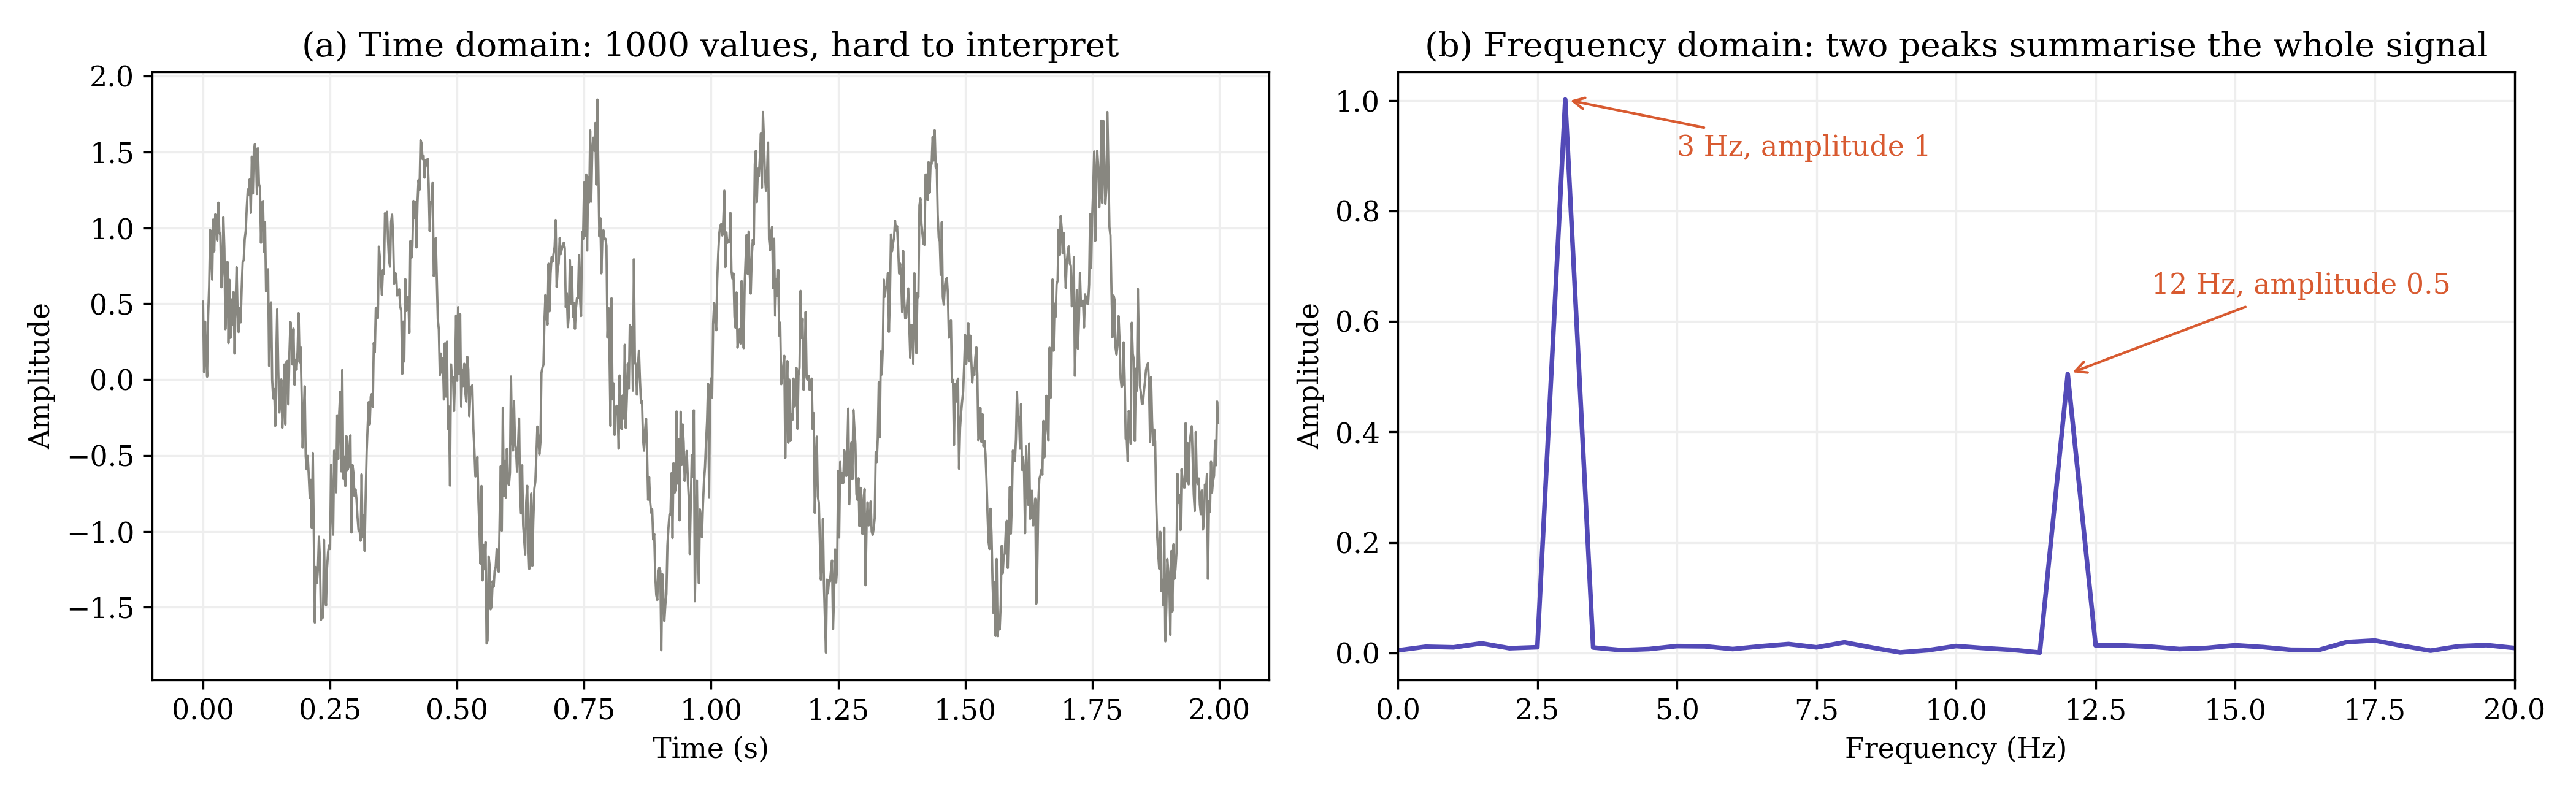
\includegraphics[width=0.8\textwidth]{images/chapter_3/fourier_transform.png}
    \caption{Fourier transform. (a) A noisy signal made of two waves (3\,Hz and 12\,Hz), represented by 1000 values over time. (b) The same signal in the frequency domain: two peaks describe it completely.}
\end{figure}

Another very common case is the conversion of \textbf{non-numerical data into numerical data}: most algorithms work only with numbers, so categories and text must be transformed (see Sections~\ref{sec:binarization} and~\ref{sec:documents}).


\subsection{Data Discretization}
Discretization converts a \textbf{continuous} attribute into an \textbf{ordinal} one: a potentially infinite number of values is mapped into a small number of ordered categories (\emph{bins}). Example: age $\in[15,90]$ $\rightarrow$ \{young, adult, senior\}. It is useful because some algorithms only accept categorical data, and because categories are often easier to interpret. The price is a loss of detail: ages 36 and 55 may end up in the same bin.

The main \textbf{unsupervised} discretization techniques (they do not use class labels) are (Figure~\ref{fig:discretization}):

\begin{figure}[htbp]
    \centering
    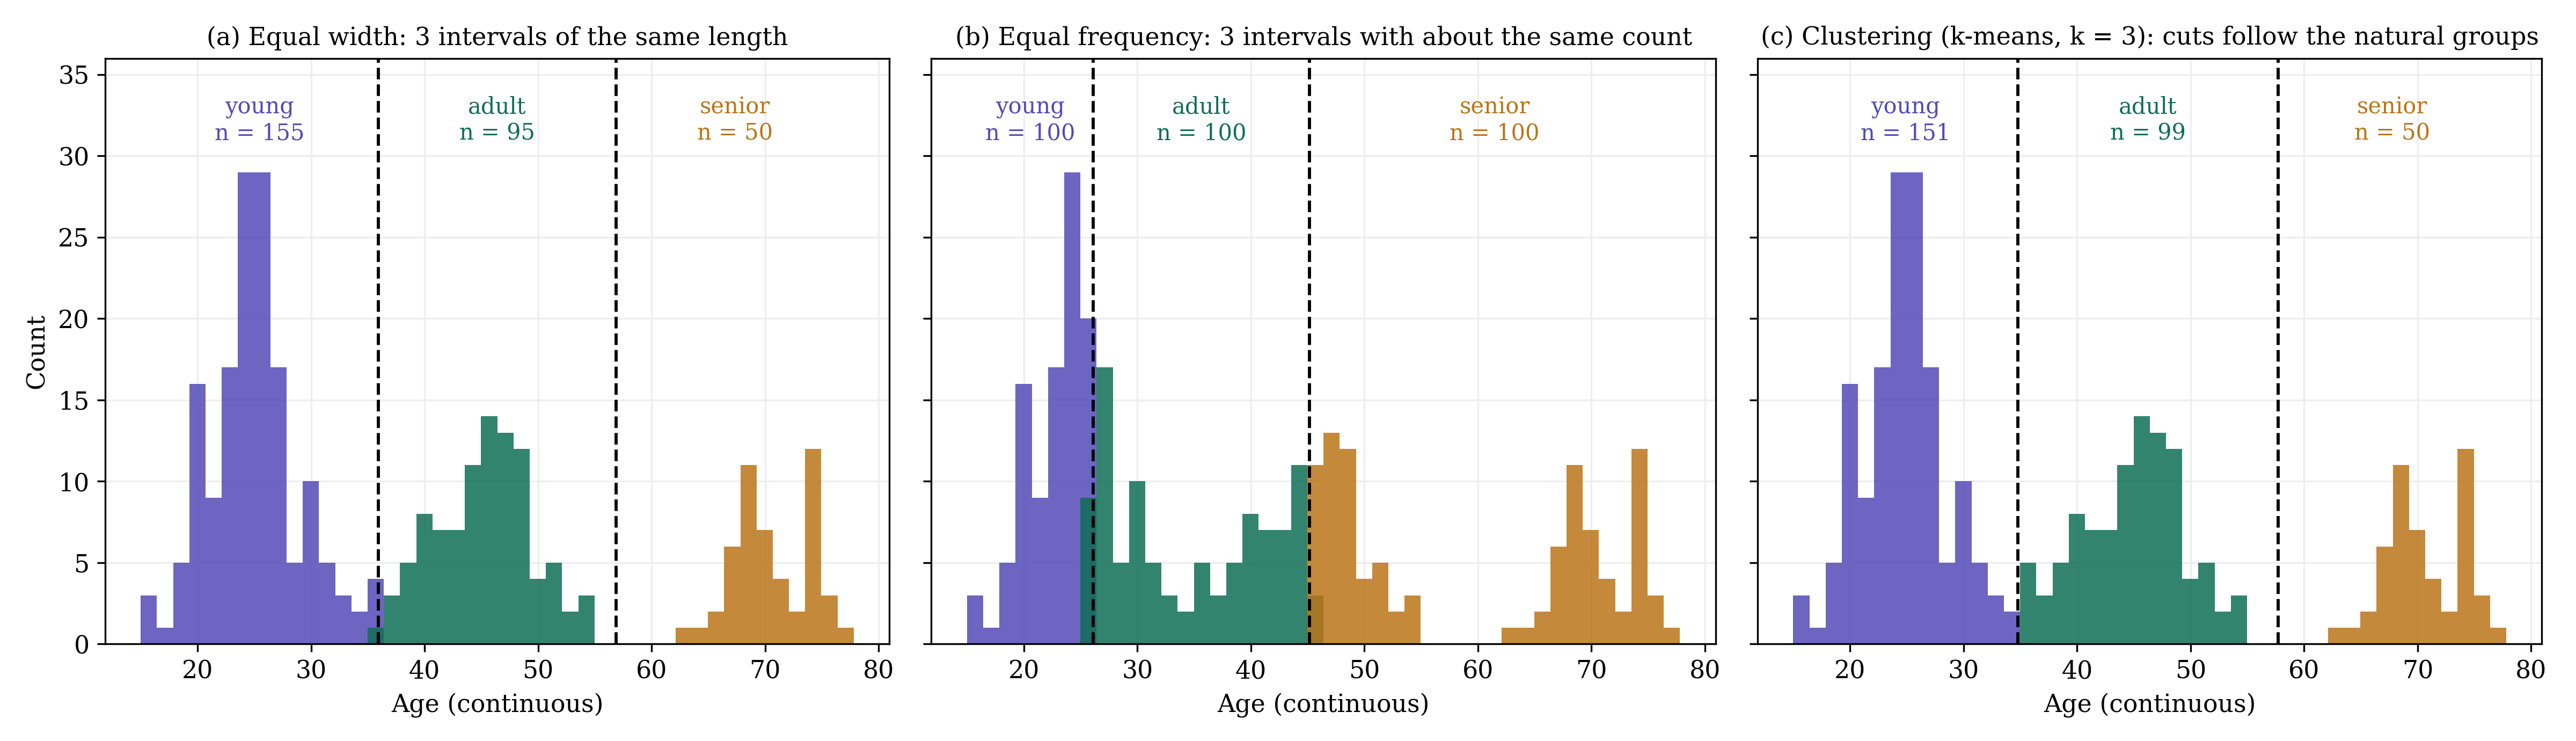
\includegraphics[width=0.8\textwidth]{images/chapter_3/discretization.png}
    \caption{Discretization of a continuous attribute (age) into 3 bins with three unsupervised techniques. The dashed lines are the cut points; each colour is one category.}
\end{figure}

\begin{itemize}
    \item \textbf{Equal width:} $N$ intervals of the same length. Simple, but some bins may contain very few points, and it is sensitive to outliers.
    \item \textbf{Equal frequency:} $N$ intervals with approximately the same number of points. Each bin is well populated, but similar values may be split into different bins.
    \item \textbf{Clustering:} the cuts are placed between natural groups of values found by a clustering algorithm (e.g.\ k-means).
\end{itemize}

\subsection{Data Binarization}
Binarization maps an attribute into one or more \textbf{binary} variables (0/1).
\begin{itemize}
    \item \textbf{Continuous attribute:} first discretize it into categories, then apply one of the techniques for categorical attributes below. Example: age $\rightarrow$ \{young, adult, senior\} $\rightarrow$ binary vector.
    \item \textbf{Categorical attribute:} map it to a set of binary attributes, for instance via \emph{one-hot encoding}.
\end{itemize}
Why not simply map the categories to integers (San Francisco $=1$, New York $=2$, Seattle $=3$)? Because the model would assume an order and a distance that do not exist (Seattle would be ``greater'' than San Francisco, and New York would be ``halfway'' between them). The following encodings avoid this problem. In all of them, a categorical variable with $k$ categories is represented by a group of bits.

\begin{itemize}
    \item \textbf{One-Hot Encoding:} one bit per category ($k$ bits). Since an object belongs to only one category, exactly one bit is set to 1. The result is a \emph{sparse} matrix (mostly zeros).
    \item \textbf{Dummy Coding:} only $k-1$ bits. One category is chosen as \emph{reference} and is encoded with all zeros; the other categories are encoded as in one-hot.
    \item \textbf{Effect Coding:} like dummy coding, but the reference category is encoded with all $-1$s instead of all $0$s.
\end{itemize}

\begin{center}
    \small
    \renewcommand{\arraystretch}{1.3}
    \begin{tabular}{|l|c|c|c||c|c||c|c|}
    \hline
     & \multicolumn{3}{c||}{\textbf{One-Hot}} & \multicolumn{2}{c||}{\textbf{Dummy}} & \multicolumn{2}{c|}{\textbf{Effect}} \\
    \hline
     & $e_1$ & $e_2$ & $e_3$ & $e_1$ & $e_2$ & $e_1$ & $e_2$ \\
    \hline
    San Francisco & 1 & 0 & 0 & 1 & 0 & 1 & 0 \\
    \hline
    New York & 0 & 1 & 0 & 0 & 1 & 0 & 1 \\
    \hline
    Seattle (reference) & 0 & 0 & 1 & 0 & 0 & $-1$ & $-1$ \\
    \hline
    \end{tabular}
\end{center}

\paragraph{Why $k-1$ bits are enough.} One-hot encoding uses $k$ bits, i.e.\ it has $k$ degrees of freedom, but the variable only needs $k-1$. In the example, if $e_1=0$ and $e_2=0$, the city \emph{must} be Seattle, so $e_3$ adds no information: it can always be computed as $e_3 = 1-e_1-e_2$. This redundancy is a problem for linear models, because the model can no longer find a unique set of coefficients (many combinations give exactly the same predictions). Dummy and effect coding remove the extra bit.

\paragraph{Pros and cons.} When these encodings are used in a linear model, they also change how the coefficients are interpreted:

\begin{center}
    \small
    \renewcommand{\arraystretch}{1.3}
    \begin{tabular}{|l|p{4.6cm}|p{4.6cm}|}
        \hline
        & \textbf{PROS} & \textbf{CONS} \\
        \hline
        \textbf{One-Hot} & each feature clearly corresponds to one category; missing data can be encoded as the all-zeros vector; the intercept of a linear model represents the overall mean of the target variable & redundant ($k$ bits for $k-1$ degrees of freedom): the linear model has no unique solution \\
        \hline
        \textbf{Dummy} & not redundant ($k-1$ bits): the solution is unique; the intercept is the mean of the target for the reference category & cannot easily handle missing data, since the all-zeros vector is already used by the reference category \\
        \hline
        \textbf{Effect} & not redundant; the reference category uses a different code ($-1$s), so the all-zeros vector is free for missing data; the intercept represents the overall mean & the vector of all $-1$s is dense (not sparse), which is expensive for both storage and computation \\
        \hline
    \end{tabular}
\end{center}

\subsection{Attribute Transformation}
An attribute transformation is a function that maps \emph{all} the values of an attribute to a new set of values, so that each old value corresponds to exactly one new value. Examples: $x \rightarrow \log x$ (to compress very skewed values), $x \rightarrow |x|$, and normalization.

\textbf{Normalization} is used to make attributes with different scales comparable. If age ranges in $[20,70]$ and income in $[20\,000,100\,000]$, any distance between two people would depend almost only on income, simply because its numbers are bigger. After normalization all attributes contribute in a comparable way. The two most common techniques are:

\begin{figure}[htbp]
    \centering
    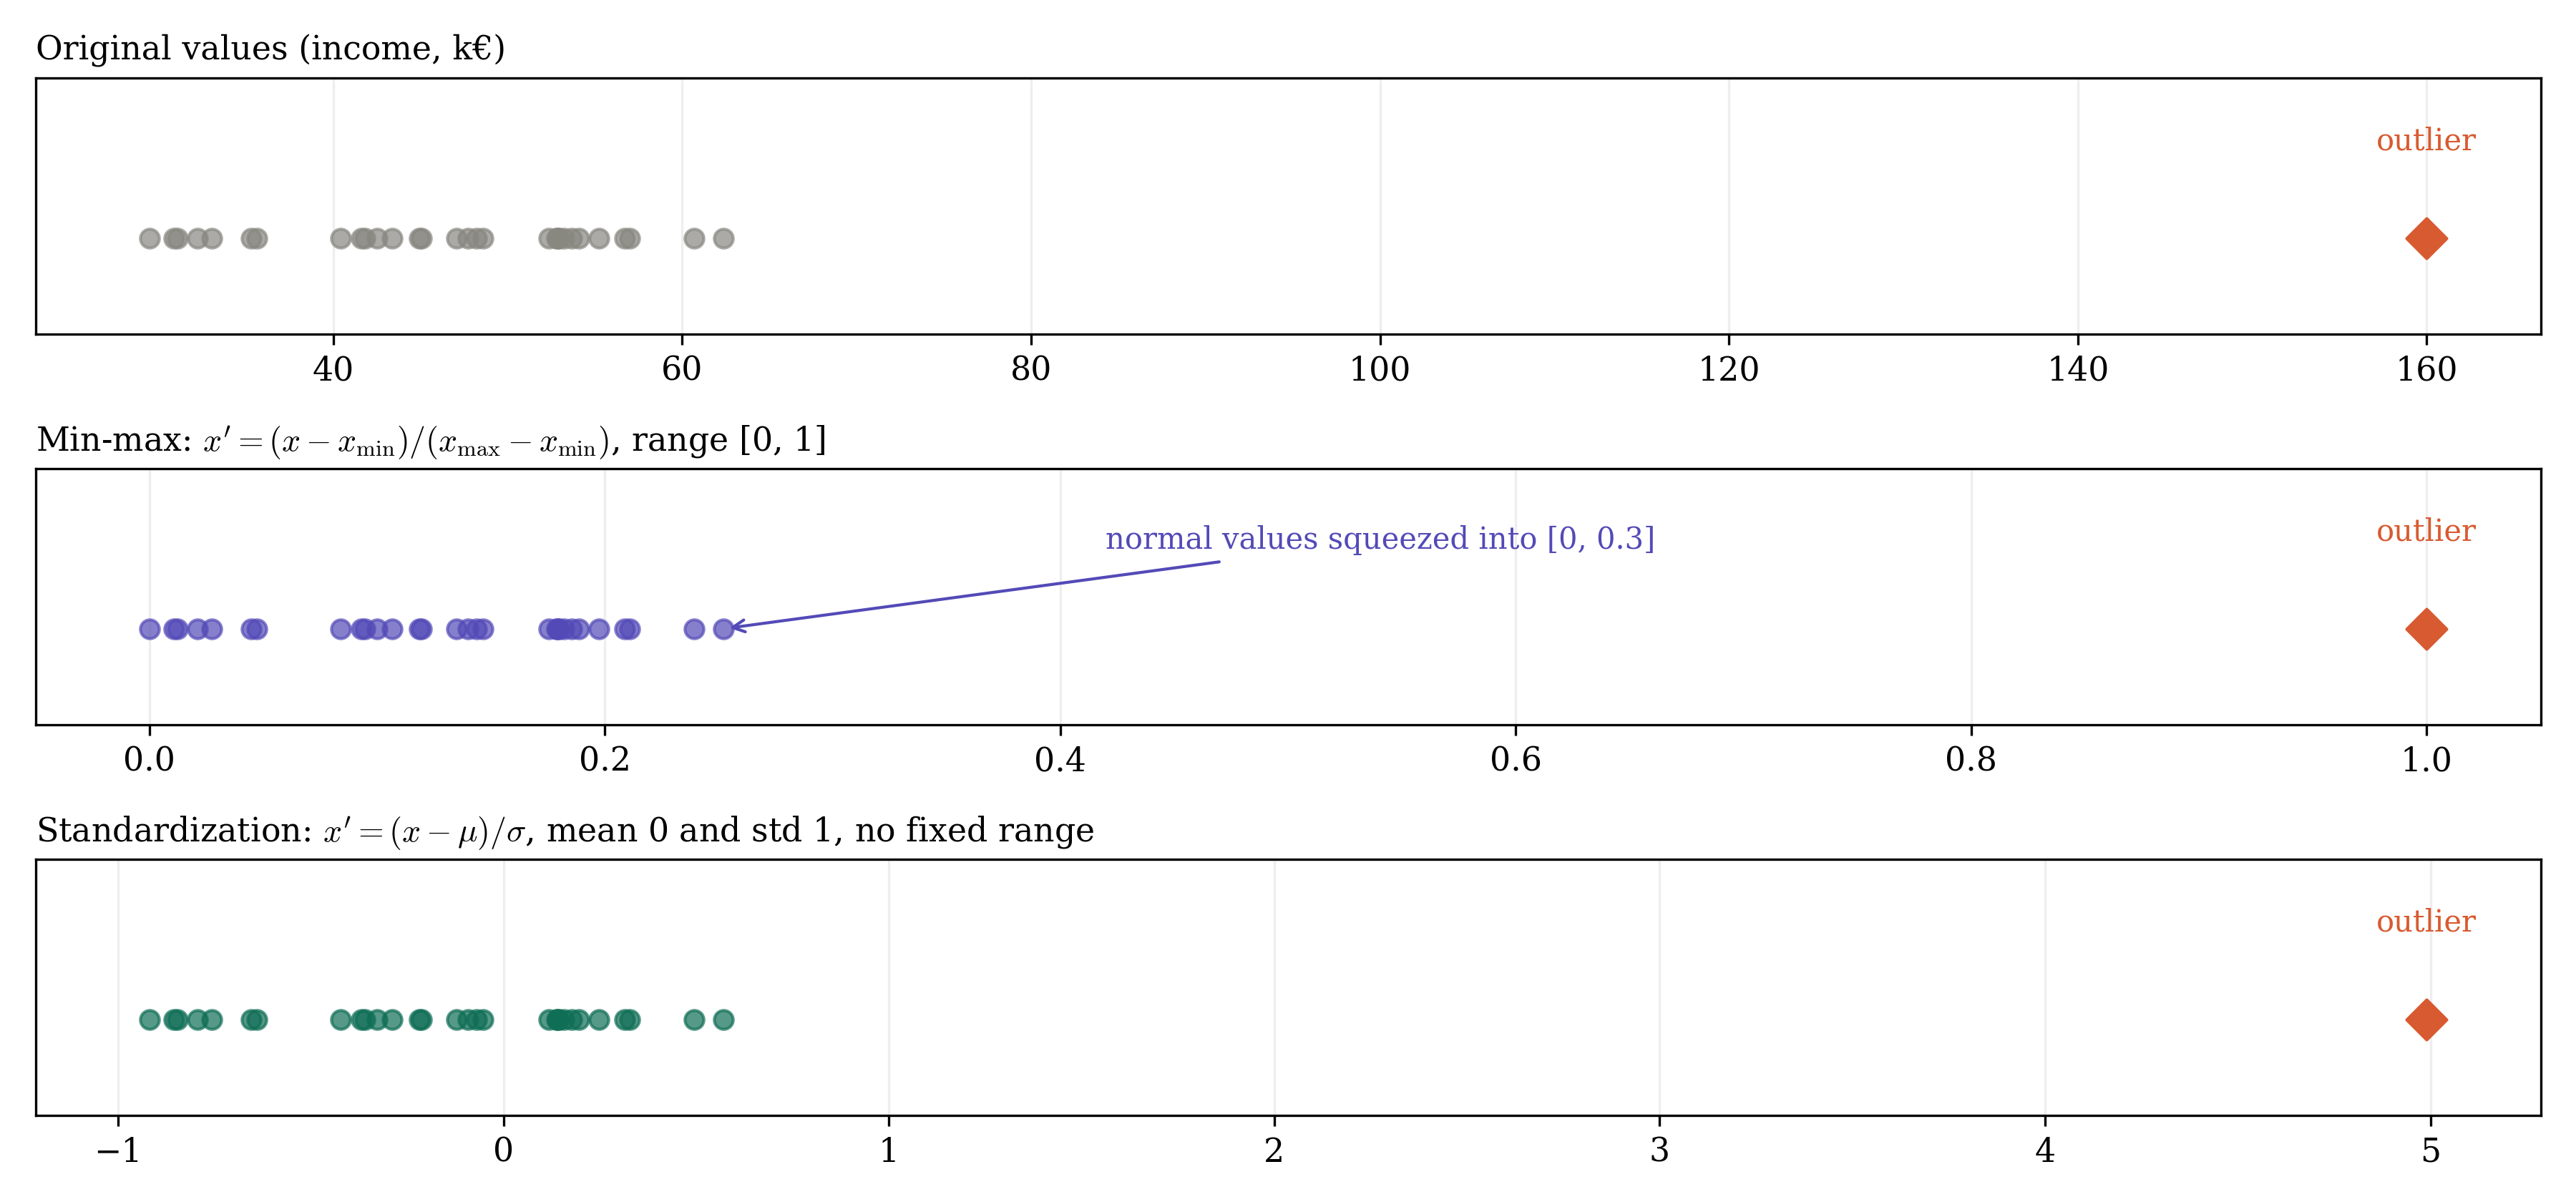
\includegraphics[width=0.9\textwidth]{images/chapter_3/normalization.png}
    \caption{Effect of normalization on data with an outlier. Min-max normalization maps the outlier to 1 and compresses all the normal values close to 0; standardization centres the data around 0 without a fixed range.}
\end{figure}

\begin{itemize}
    \item \textbf{Min-Max Normalization:} rescales the values linearly into the range $[0,1]$: the minimum becomes $0$ and the maximum becomes $1$.
    \[
        x'=\frac{x-x_{\min}}{x_{\max}-x_{\min}}
    \]
    It retains the shape of the distribution, but it is \textbf{sensitive to outliers}: a single extreme value becomes the maximum and squeezes all the other values into a small part of the range (Figure~\ref{fig:normalization}). Example: with $x_{\min}=20$ and $x_{\max}=70$, the value $x=45$ becomes $x'=25/50=0.5$.
    \item \textbf{Standardization (z-score):} subtracts the mean $\mu$ and divides by the standard deviation $\sigma$, so that the new values have zero mean and unit standard deviation.
    \[
        x'=\frac{x-\mu}{\sigma}
    \]
    The new value tells \emph{how many standard deviations} $x$ is from the mean. It is not bounded to a fixed range, and outliers remain clearly visible as large values. Example: with $\mu=50$ and $\sigma=10$, the value $x=70$ becomes $x'=2$.
\end{itemize}


\noindent\textbf{Note:} the parameters ($x_{\min}$, $x_{\max}$, $\mu$, $\sigma$) must be computed on the training data only, and then applied unchanged to the test data.

\subsection{Data Preparation for Document Data}
Most algorithms cannot process raw text directly: they need numbers. For this reason a document is usually represented as a set of features. \textbf{Document PreProcessing} is the activity that generates a structured representation of documents, and it includes five sequential steps:
\begin{enumerate}
    \item \textbf{Document Splitting:} depending on the goal of the analysis, documents are split into sentences or paragraphs, or analysed in their entire content.
    \item \textbf{Tokenization:} breaking the text into units called \emph{tokens}, typically words, for instance by separating words at spaces and identifying sentence boundaries based on punctuation.
    \item \textbf{Case Normalization:} converting every token to lower-case (or upper-case), so that ``The'' and ``the'' are treated as the same word.
    \item \textbf{Stopword Elimination:} removing \emph{stopwords}, the most common words of a language (articles, prepositions, auxiliary verbs, \dots), which appear everywhere and carry little meaning.
    \item \textbf{Stemming:} reducing each word to its root (\emph{stem}), so that different forms of the same word are counted together: ``running'', ``runs'' $\rightarrow$ ``run''; ``cats'' $\rightarrow$ ``cat''.
\end{enumerate}

The following example shows how one sentence changes at each step:

\begin{center}
    \small
    \renewcommand{\arraystretch}{1.3}
    \begin{tabular}{|l|p{7.7cm}|}
    \hline
    \textbf{Step} & \textbf{Result} \\
    \hline
    Original text & \texttt{The cats are running in the garden. The dog runs and the dog barks.} \\
    \hline
    1. Splitting & S1: \texttt{The cats are running in the garden.} \newline S2: \texttt{The dog runs and the dog barks.} \\
    \hline
    2. Tokenization (S1) & \texttt{[The, cats, are, running, in, the, garden]} \\
    \hline
    3. Case normalization & \texttt{[the, cats, are, running, in, the, garden]} \\
    \hline
    4. Stopword elimination & \texttt{[cats, running, garden]} \\
    \hline
    5. Stemming & \texttt{[cat, run, garden]} \\
    \hline
    \end{tabular}
\end{center}

\paragraph{Term vectors (bag of words).} After preprocessing, each document is represented as a \textbf{term vector}: each distinct term is an attribute, and the value of the attribute is the number of times the term occurs in the document. The order of the words is ignored. Putting all the vectors together gives the \textbf{document-term matrix}. Example with three short documents:
\begin{itemize}
    \item $D_1$: ``The cats are running in the garden'' $\rightarrow$ \{cat, run, garden\}
    \item $D_2$: ``The dog runs and the dog barks'' $\rightarrow$ \{dog, run, dog, bark\}
    \item $D_3$: ``A dog and a cat in the garden'' $\rightarrow$ \{dog, cat, garden\}
\end{itemize}

\begin{center}
    \small
    \renewcommand{\arraystretch}{1.3}
    \begin{tabular}{|l|c|c|c|c|c|}
    \hline
     & \textbf{bark} & \textbf{cat} & \textbf{dog} & \textbf{garden} & \textbf{run} \\
    \hline
    $D_1$ & 0 & 1 & 0 & 1 & 1 \\
    \hline
    $D_2$ & 1 & 0 & 2 & 0 & 1 \\
    \hline
    $D_3$ & 0 & 1 & 1 & 1 & 0 \\
    \hline
    \end{tabular}
\end{center}

\paragraph{Weighting schemes.} The value of each term can be computed in different ways:
\begin{itemize}
    \item \textbf{Binary:} $1$ if the term appears in the document, $0$ otherwise.
    \item \textbf{Term Frequency (TF):} the number of occurrences of the term in the document (as in the table above).
    \item \textbf{TF-IDF:} the term frequency multiplied by a factor that rewards rare terms and penalises terms that appear in many documents:
    \[
        \text{tf-idf}(t,d)=\text{tf}(t,d)\cdot\log\frac{N}{\text{df}(t)}
    \]
    where $N$ is the number of documents and $\text{df}(t)$ is the number of documents containing term $t$. A term that appears in every document gets weight $\log 1 = 0$, because it does not help to distinguish documents. In the example ($N=3$, natural logarithm), ``bark'' appears only in $D_2$, so its weight is $1\cdot\log 3\approx1.10$, while ``dog'' appears in two documents and gets $2\cdot\log 1.5\approx0.81$ in $D_2$, even though it occurs twice.
\end{itemize}


\section{A prova di coglione}

\subsection*{Attributi e dati}
Un \textbf{attributo} è una caratteristica (es.\ l'altezza), il \textbf{valore} è il modo in cui la misuriamo (metri o piedi). Lo stesso attributo può avere valori diversi, e attributi diversi possono avere gli stessi valori (ID ed età sono entrambi interi).

\begin{center}
\small
\begin{tabular}{@{}lll@{}}
\toprule
\textbf{Tipo} & \textbf{Cosa posso fare} & \textbf{Esempio} \\
\midrule
Nominale & solo dire se sono uguali ($=$) & colore degli occhi, ID \\
Ordinale & uguali e ordinarli ($<,=,>$) & voti, taglie S/M/L \\
Discreto & pochi valori, spesso interi (binario = caso speciale) & conteggi, 0/1 \\
Continuo & numeri reali & altezza, temperatura \\
\bottomrule
\end{tabular}
\end{center}

\noindent I dati possono essere \textbf{tabelle}, \textbf{documenti} (testo), \textbf{grafi} (il Web) o \textbf{dati ordinati} (serie temporali, genoma).

\paragraph*{Qualità.} Ogni dataset ha dei difetti:
\begin{itemize}
    \item \textbf{Rumore}: valori alterati a caso (es.\ errori di misura). \textbf{Outlier}: oggetti molto diversi dagli altri; a volte disturbano, a volte sono proprio ciò che cerchiamo.
    \item \textbf{Valori mancanti}: si eliminano, si stimano o si ignorano.
    \item \textbf{Duplicati}: tipici quando si uniscono più fonti; vanno ripuliti.
\end{itemize}

\subsection*{Similarità e distanza}
La \textbf{dissimilarità} $d$ vale $0$ se due oggetti sono identici e cresce quanto più sono diversi. La \textbf{similarità} $s$ fa l'opposto: di solito sta in $[0,1]$ e vale $1$ per oggetti identici.

\paragraph*{Un solo attributo.}
\begin{itemize}
    \item \textbf{Nominale}: o uguali ($d=0$) o diversi ($d=1$), senza vie di mezzo.
    \item \textbf{Ordinale}: si numerano i valori da $0$ a $n-1$ e $d=\frac{|x-y|}{n-1}$, $s=1-d$. Con \{poor, fair, good, excellent\}: $d(\text{poor},\text{good})=2/3$. Si assume che i ``gradini'' siano tutti uguali.
    \item \textbf{Numerico}: $d=|x-y|$. Per la similarità: $s=-d$, $s=\frac{1}{1+d}$, $s=e^{-d}$ oppure min-max. Con $d=2$: $-2$, $0.33$, $0.14$.
\end{itemize}

\paragraph*{Più attributi: Minkowski.} Ogni oggetto è un punto in $n$ dimensioni e
\[
d(\mathbf{x},\mathbf{y})=\Big(\sum_{k=1}^{n}|x_k-y_k|^r\Big)^{1/r}
\]
Il parametro $r$ (scelto da noi, non è $n$) decide come combinare le differenze:
$r=1$ \textbf{Manhattan} (somma delle differenze, come camminare tra isolati),
$r=2$ \textbf{Euclidea} (linea retta),
$r\to\infty$ \textbf{Chebyshev} (solo la differenza più grande).
Esempio: $\mathbf{x}=(1,1)$, $\mathbf{y}=(4,5)$, differenze $3$ e $4$ $\Rightarrow$ $L_1=7$, $L_2=5$, $L_\infty=4$.
Se gli attributi hanno scale diverse (euro vs anni) vince quello con i numeri più grandi: prima si \textbf{standardizza}.

\paragraph*{Quando una distanza è una metrica.} Deve rispettare: $d(x,x)=0$; $d(x,y)>0$ se $x\neq y$; $d(x,y)=d(y,x)$; e la \textbf{disuguaglianza triangolare} $d(x,z)\le d(x,y)+d(y,z)$ (la strada diretta non è mai più lunga di una deviazione). Minkowski è una metrica solo per $r\ge1$: con $r=0.5$, $x=(0,0)$, $y=(1,0)$, $z=(1,1)$ si ottiene $d(x,z)=4 > 1+1$.

\paragraph*{Mahalanobis.} Idea: \emph{una differenza pesa tanto quanto è insolita}.
\[
d(\mathbf{x},\mathbf{y})=\sqrt{(\mathbf{x}-\mathbf{y})^\top S^{-1}(\mathbf{x}-\mathbf{y})}
\]
dove $S$ è la matrice di covarianza. Dove i dati variano molto, una differenza conta poco; dove variano poco, conta molto. Tiene conto anche delle correlazioni, così le informazioni ripetute non contano due volte. Non dipende dalle unità di misura. Se $S=I$ torna la distanza euclidea; se $S$ è diagonale equivale all'euclidea su dati standardizzati.
Esempio con varianze $4$ e $1$: la differenza $(2,0)$ dà $d=1$, la differenza $(0,2)$ dà $d=2$. Stessa distanza euclidea, ma la seconda è più ``strana''.

\subsection*{Preprocessing}
I dati reali sono sporchi, enormi, con troppi attributi o non numerici. Il preprocessing li rende puliti, compatti e utilizzabili.

\paragraph*{Aggregazione.} Più valori diventano uno solo (somma o media): giorni $\to$ mesi, città $\to$ regioni. Si ottengono meno dati, una visione d'insieme e valori più stabili (nella media le oscillazioni si compensano). Si perde però il dettaglio.

\paragraph*{Riduzione.} Un dataset più piccolo che dà quasi gli stessi risultati: \textbf{meno righe} (campionamento), \textbf{meno colonne} (selezione delle feature), \textbf{meno valori} (discretizzazione).

\paragraph*{Campionamento.} Si analizza solo una parte dei dati, che deve essere \textbf{rappresentativa} (stesse medie, stesse proporzioni delle classi).
\textbf{Casuale semplice}: tutti hanno la stessa probabilità, ma una classe rara può sparire per caso.
\textbf{Stratificato}: si campiona da ogni gruppo in proporzione alla sua dimensione, così nessuna classe si perde.

\paragraph*{Maledizione della dimensionalità.} Con tante dimensioni lo spazio diventa enorme e i dati \textbf{vuoti e sparsi}. Per prendere il 10\% dei dati in un cubo serve un lato di $0.1$ in 1D, ma di $0.79$ in 10D: il ``vicino'' non è più vicino. Inoltre tutti i punti diventano quasi equidistanti, quindi distanza e densità (base di clustering e outlier detection) perdono senso.

\paragraph*{Selezione delle feature.} Si tolgono feature \textbf{ridondanti} (prezzo con e senza IVA) e \textbf{irrilevanti} (la matricola per prevedere il voto). Metodi:
\begin{itemize}
    \item \textbf{RFE}: addestro il modello, elimino la feature meno importante, riaddestro, ripeto fino al numero voluto. Si riaddestra ogni volta perché le importanze cambiano; per questo è lento con molte feature.
    \item \textbf{Modelli interpretabili}: alberi di decisione e regressione lineare dicono già quanto pesa ogni feature.
    \item \textbf{PCA/SVD}: non scelgono feature, ne \emph{creano} di nuove combinando le originali; poche componenti contengono quasi tutta l'informazione.
\end{itemize}

\paragraph*{Feature engineering.} Trasformare i dati grezzi nella forma più utile al modello: spesso conta più dell'algoritmo. Dati strutturati $\to$ normalizzazione, discretizzazione, binarizzazione; testo, immagini, segnali $\to$ tokenizzazione, Fourier, descrittori.

\paragraph*{Trasformazione.} Cambiare rappresentazione per far emergere l'informazione. Esempio: la \textbf{trasformata di Fourier} trasforma un segnale di 1000 valori nel tempo in due soli picchi di frequenza.

\paragraph*{Discretizzazione.} Da continuo a categorie ordinate: età $\to$ \{giovane, adulto, anziano\}. Più facile da interpretare, ma si perde dettaglio.
\textbf{Equal width}: intervalli della stessa ampiezza (semplice, sensibile agli outlier).
\textbf{Equal frequency}: stesso numero di punti per intervallo.
\textbf{Clustering}: tagli tra i gruppi naturali (es.\ k-means).

\paragraph*{Binarizzazione.} Le categorie diventano bit. Non si usano numeri (SF=1, NY=2, Seattle=3) perché inventerebbero un ordine che non esiste.
\begin{center}
    \small
    \begin{tabular}{@{}l|ccc|cc|cc@{}}
        \toprule
        & \multicolumn{3}{c|}{\textbf{One-hot}} & \multicolumn{2}{c|}{\textbf{Dummy}} & \multicolumn{2}{c}{\textbf{Effect}} \\
        \midrule
        San Francisco & 1 & 0 & 0 & 1 & 0 & 1 & 0 \\
        New York      & 0 & 1 & 0 & 0 & 1 & 0 & 1 \\
        Seattle       & 0 & 0 & 1 & 0 & 0 & $-1$ & $-1$ \\
        \bottomrule
    \end{tabular}
\end{center}

Il \textbf{one-hot} usa $k$ bit, ma uno è inutile: se i primi due sono $0$, la città è per forza Seattle. Questo confonde i modelli lineari (nessuna soluzione unica). \textbf{Dummy} ed \textbf{effect} usano $k-1$ bit e risolvono il problema.
In breve: \emph{one-hot} è chiaro e gestisce i mancanti (vettore nullo) ma è ridondante; \emph{dummy} non è ridondante ma il vettore nullo è già occupato; \emph{effect} risolve entrambi, ma i $-1$ rendono i dati densi e costosi.

\paragraph*{Normalizzazione.} Rende confrontabili scale diverse (età 20--70 vs reddito 20\,000--100\,000).
\begin{itemize}
    \item \textbf{Min-max}: $x'=\frac{x-x_{\min}}{x_{\max}-x_{\min}}\in[0,1]$. Un outlier però schiaccia tutti gli altri valori verso $0$.
    \item \textbf{Z-score}: $x'=\frac{x-\mu}{\sigma}$, cioè ``a quante deviazioni standard dalla media''. Gli outlier restano visibili.
\end{itemize}
Media, min e max si calcolano \textbf{solo sul training set}.

\paragraph*{Documenti.} Il testo va trasformato in numeri in cinque passi:
\begin{center}
    \small
    \texttt{The cats are running in the garden.}
    $\xrightarrow{\text{token}}$ \texttt{[The, cats, are, running, in, the, garden]}\\[2pt]
    $\xrightarrow{\text{minuscolo}}$ \texttt{[the, cats, \dots]}
    $\xrightarrow{\text{via stopword}}$ \texttt{[cats, running, garden]}
    $\xrightarrow{\text{stemming}}$ \texttt{[cat, run, garden]}
    \end{center}
    (il primo passo, lo \emph{splitting}, divide il testo in frasi o paragrafi). Poi ogni documento diventa un vettore che conta le parole (\textbf{bag of words}), ignorandone l'ordine:
    \begin{center}
    \small
    \begin{tabular}{@{}lccccc@{}}
    \toprule
    & bark & cat & dog & garden & run \\
    \midrule
    $D_1$: The cats are running in the garden & 0 & 1 & 0 & 1 & 1 \\
    $D_2$: The dog runs and the dog barks & 1 & 0 & 2 & 0 & 1 \\
    $D_3$: A dog and a cat in the garden & 0 & 1 & 1 & 1 & 0 \\
    \bottomrule
    \end{tabular}
\end{center}

I pesi possono essere \textbf{binari} (c'è o no), \textbf{TF} (quante volte) o \textbf{TF-IDF}, che premia le parole rare:
\[
\text{tf-idf}(t,d)=\text{tf}(t,d)\cdot\log\frac{N}{\text{df}(t)}
\]
Una parola presente in tutti i documenti pesa $0$, perché non aiuta a distinguerli. Nell'esempio ``bark'' vale $\log 3\approx1.10$, mentre ``dog'' vale solo $0.81$ pur comparendo due volte.